% Imperial College ACSE 2019/20 IRP Report
\documentclass[%
   %draft,     % faster rendering with grayscale only, no active links, placeholders for figures
   final,      % final document
%%%% --- font size ---
   fontsize=11pt,
   headings=small,
   %headings=normal,
   %headings=big,
%%%% --- Language ---
   british,          % forwarded to other packages
%%%% === Page size ===
   paper=a4,         % letter, legal, executive, a4, a5
   % landscap,
%%%% === Options for text positioning ===
   BCOR=5mm,          % More margin on the book inside if twosided
   DIV=15,            % page size (see Koma Skript docs!)
   headlines=1.1,     % num lines in header
   headinclude=false,% include header in page size
   footinclude=false,% include footer in page size
   mpinclude=false,  % include margin in page size
   pagesize,         % writes page dimensions into pdf file; important for conversions
%%%% === Layout ===
   oneside,
   %twoside,
   %onecolumn,
   twocolumn,
   %openany,         % start chapter on any side
   %openright,       % start chapter only on right any side
                     % (macht nur bei 'twoside' Sinn)
   %cleardoubleplain,% leere, linke Seite mit Seitenstil 'plain'
   %cleardoubleempty,% leere, linke Seite mit Seitenstil 'empty'
   %titlepage,        % title as separate page (use 'titlepage' environment)
   notitlepage,     % include title on first page
%%%% --- Paragraph indentation ---
   %                 % Absatzabstand: Einzeilig,
   %parskip,         % Freiraum in letzter Zeile: 1em
   %parskip*,        % Freiraum in letzter Zeile: Viertel einer Zeile
   %parskip+,        % Freiraum in letzter Zeile: Drittel einer Zeile
   %parskip-,        % Freiraum in letzter Zeile: keine Vorkehrungen
   %                 % Absatzabstand: Halbzeilig
   %halfparskip,     % Freiraum in letzter Zeile: 1em
   %halfparskip*,    % Freiraum in letzter Zeile: Viertel einer Zeile
   %halfparskip+,    % Freiraum in letzter Zeile: Drittel einer Zeile
   %halfparskip,     % Freiraum in letzter Zeile: keine Vorkehrungen
   %                 % Absatzabstand: keiner
   parskip=false,    % Eingerueckt (Standard)
                     % true, full-,full+, full*, half, half-,half+,half*                                    
%%%% --- Kolumnentitel ---
   %headsepline,      % Linie unter Kolumnentitel
   headsepline=false, % keine Linie unter Kolumnentitel
   %footsepline,     % Linie unter Fussnote
   %footnosepline,   % keine Linie unter Fussnote
%%%% --- Kapitel ---
   %chapterprefix,   % Ausgabe von 'Kapitel:'
   %nochapterprefix,  % keine Ausgabe von 'Kapitel:'
%%%% === Verzeichnisse (TOC, LOF, LOT, BIB) ===
   %toc=listof,      % Tabellen & Abbildungsverzeichnis ins TOC   
   %toc=index,       % Index ins TOC
   %toc=left,        % Tabellenartige TOC
   toc=graduated,    % eingereuckte Gliederung
   bibliography=totoc,% Bibliographie ins TOC
   %toc=bibnumbered, % Bibliographie im TOC nummeriert
   toc=listofnumbered, % Alle Verzeichnisse im TOC nummeriert
   listof=graduated, % eingereuckte LOT, LOF
   %listsleft,       % Tabellenartige LOT, LOF
   %pointednumbers,  % Ueberschriftnummerierung mit Punkt, siehe DUDEN !
   numbers=noenddot, % Ueberschriftnummerierung ohne Punkt, siehe DUDEN !
   %openbib,         % alternative Formatierung des Literaturverzeichnisses
%%%% === Matheformeln ===
   %leqno,           % Formelnummern links
   %fleqn,            % Formeln werden linksbuendig angezeigt
]{scrartcl}%     Klassen: scrartcl, scrreprt, scrbook

% Packages
../../preamble.tex

% title page
\titlehead{\centering ACSE-9 Independent Research Project}
\title{Inversion of Meteoroid Properties from \\
       Impact Crater Clusters on Mars \\
       with a Fragment-Cloud Model}
\author{\small Dominic Schwarz \\
        \small dominic.schwarz19@imperial.ac.uk \\
        \small \url{github.com/acse-ds2419}}
\date{\today}
%\uppertitleback{\copyright 2014 D. Hennig}
%\lowertitleback{Ubuntu-Version}
\publishers{\small{%
   \vspace{2em}
   Imperial College London \\
   Royal School of Mines \\
   Department of Earth Science and Engineering \\
   \vspace{2em}
   Supervisor: \\
   Prof. Gareth Collins \\
   g.collins@imperial.ac.uk \\
   \vspace{2em}
   Project repository: \\
   \url{https://github.com/acse-2019/irp-acse-ds2419} \\
   \vspace{2em}
   Submitted as part of the MSc course in \\
   Applied Computational Science and Engineering. \\
}
}
%\dedication{Widmung}
%\extratitle{Schmutztitel}

\begin{document}

%%% Settings that need to be made after begin{document}
\renewcommand\bf{\bfseries}  % fix for natbib using deprecated \bf command
\setlength{\parindent}{1.5em} % paragraph indentation

%%% Command definitions %%%
\newcommand{\unit}[1]{\,\mathrm{#1}}
\newcommand{\e}[1]{\cdot 10^{#1}}
\newcommand{\intd}[1]{\,\mathrm{d}#1}
\newcommand{\parnorm}[1]{\frac{\partial}{\partial #1}}
\newcommand{\parnormp}[2]{\frac{\partial^#2}{\partial #1^#2}}
\newcommand{\parfrac}[2]{\frac{\partial #1}{\partial #2}}
\newcommand{\parfracp}[3]{\frac{\partial^#3 #1}{\partial #2^#3}}


%%% Titlepage %%%
\onecolumn{
    \maketitle
    \begin{abstract}
        \noindent
        Analysis of impact craters on bodies within the solar system can give insight into properties of meteoroids forming these craters.
While there are empirical relationships for estimating the size of a crater from impactor properties and vice versa \citep[e.g.][]{holsapple1987scaling}, these relationships are not directly applicable to small impacts on planets with an atmosphere.
When impacting these planets, small-sized meteoroids experience significant deceleration, mass loss due to ablation, and potential break up before impacting the ground.
As a result of these processes, they typically produce clusters of impact craters, or only leave a strewn field of small meteorites if most of their kinetic energy has been deposited in the atmosphere.
Impact crater clusters are much more prevalent on Mars than on Earth due to the much thinner martian atmosphere. \cite{daubar2019recently} collected a set of 77 recently formed crater clusters and studied a couple of their characteristics.
In this work, we develop a high-performance atmospheric entry model that computes the spatial distribution and size of impact craters produced by a meteoroid.
We study characteristics by which two clusters can be compared, and we study the applicability of a Markov chain Monte Carlo inversion method for finding meteoroid features for which the model produces clusters with similar characteristics compared to a given image of a real cluster.

    \end{abstract}
}

%%% Manual Titlepage %%%

%\thispagestyle{plain}
%\vspace*{1cm}
%\begin{center}
%	\Huge{Description of Galactic, Star Forming Disks with the Accretion Disk Formalism}\\[1cm]
%	\Large{Dominic Schwarz}\\
%	\emph{ETH Z\"urich}\\[.7cm]
%	\today\\[3cm]
	
%	\section*{\large Abstract}
%\end{center}

%Analysis of impact craters on bodies within the solar system can give insight into properties of meteoroids forming these craters.
While there are empirical relationships for estimating the size of a crater from impactor properties and vice versa \citep[e.g.][]{holsapple1987scaling}, these relationships are not directly applicable to small impacts on planets with an atmosphere.
When impacting these planets, small-sized meteoroids experience significant deceleration, mass loss due to ablation, and potential break up before impacting the ground.
As a result of these processes, they typically produce clusters of impact craters, or only leave a strewn field of small meteorites if most of their kinetic energy has been deposited in the atmosphere.
Impact crater clusters are much more prevalent on Mars than on Earth due to the much thinner martian atmosphere. \cite{daubar2019recently} collected a set of 77 recently formed crater clusters and studied a couple of their characteristics.
In this work, we develop a high-performance atmospheric entry model that computes the spatial distribution and size of impact craters produced by a meteoroid.
We study characteristics by which two clusters can be compared, and we study the applicability of a Markov chain Monte Carlo inversion method for finding meteoroid features for which the model produces clusters with similar characteristics compared to a given image of a real cluster.

%\clearpage


%%% Table of Contents %%%

%\setlength{\parskip}{0em}
%\linespread{1.0}
%\tableofcontents
%\setlength{\parskip}{0.3em}
%\linespread{1.1}
%\clearpage


%%% Content %%%
\twocolumn{
\section{Introduction}
Analysis of impact craters on bodies within the solar system can give insight into properties of meteoroids forming these craters.
While there are empirical relationships for estimating the size of a crater from impactor properties and vice versa \citep[e.g.][]{holsapple1987scaling}, these relationships are not directly applicable to small impacts on planets with an atmosphere.
When impacting these planets, small-sized meteoroids experience significant deceleration, mass loss due to ablation, and potential break up before impacting the ground.
As a result of these processes, they typically produce clusters of impact craters, or only leave a strewn field of small meteorites if most of their kinetic energy has been deposited in the atmosphere.

The aim of this project is to invert impactor properties from data in a recent survey of Martian impact crater clusters \citep{daubar2019recently}.
We will investigate whether stochastic inversion methods, such as Markov Chain Monte Carlo (MCMC), are a viable approach for this problem.
MCMC models, such as the Gibbs sampler combined with the Metropolis-Hastings algorithm \citep{gelfand1990sampling}, have been a very popular black box inversion method in many research areas \citep[e.g., in epidemiology][]{flaxman2020estimating}.
In order to use an MCMC method, a high-performance numerical model of atmospheric descent and crater cluster formation is needed.

A popular way of modeling these processes is to build on the standard meteor physics equations of motion and ablation \citep[e.g.][]{opik1958physics}, which are a set of ordinary differential equations (ODEs) treating the meteoroid as a homogeneous, spherical or ellipsoidal body.
Break up is modeled to occur when the pressure difference between the leading edge and the trailing edge of the meteoroid exceeds the aerodynamic strength of the meteoroid material.
% The pressure at the leading edge, behind the bow shock, is called the stagnation pressure. The pressure on the other end, in the meteoroid wake, is nearly zero \citep{passey1980effects}.
The exact mechanism of break up is subject to ongoing research. Most break up models use either a ``pancake'' approach, or a discrete fragmentation approach \citep{register2017asteroid}.
% \cite{hills1993fragmentation} for example used a pancake approach to model energy deposition and airburst damage for various impactors on Earth. The discrete fragmentation approach was used for example by \cite{passey1980effects} to investigate strewn fields on Earth.

More recently, a combination of the two approaches, called the fragment-cloud model (FCM), was proposed by \cite{wheeler2017fragmentcloud}.
The concept behind this model was first presented by \cite{mehta2015break}.
It combines the separate-wake fragments model \citep{passey1980effects,artemieva1996interaction} with a pancake-like model:
When the meteoroid's strength is exceeded, it splits into a debris cloud plus several discrete fragments, which are all treated independently from each other after separation.
In a subsequent publication, \cite{wheeler2018atmospheric} were able to demonstrate excellent agreement between simulated energy deposition and that inferred from light curves of four recent meteoroid impacts on Earth.
% They extended their FCM from the previous publication, enabling it to represent meteoroids with varied initial structures, such as rubble piles or fractured bodies. Their model was the first to successfully replicate spikes in the energy deposition curves, representing flashes in the light curve observations that they studied.

\cite{newland2019CFM18} applied the FCM model and key conclusions from the \cite{wheeler2018atmospheric} paper to the formation of impact crater clusters on Mars.
They were able to demonstrate that the FCM model, with the right parameters, was able to reproduce crater clusters with a similar distribution of certain characteristics compared to observations collected by \cite{daubar2019recently}.
They also showed that simpler models, like the discrete fragmentation approach or the FCM model without varied initial structures, as first proposed by \cite{wheeler2017fragmentcloud}, were unable to reproduce the observed distributions of cluster characteristics.

Based on these promising results, we will use the FCM model for our inversion problem.
However, a key downside of MCMC inversion methods is their heavy computational costs.
They typically run the underlying model thousands of times to generate an accurate input space distribution.
In our case, the underlying FCM model is computationally demanding in its own right.
Equations for potentially hundreds of fragments and debris clouds have to be solved numerically for each impact.

The FCM implementation by \cite{newland2019CFM18} was based in pure Python.
A single simulation run took on the order of seconds to tens of seconds, and was limited, by nature of its pure Python implementation, to be single-threaded.
To facilitate fast iteration and realistic, scalable run times for the inversion problem, we aim to develop an open source FCM implementation in a fast, compiled language, C++, along with a Python API.
We expect the performance to increase by at least two orders of magnitude from this switch on its own.
If time permits, we will investigate further optimisations.


\section{Forward Model}
\label{sec:forward_model}
The modelling framework developed here builds on the work by \cite{wheeler2017fragmentcloud,wheeler2018atmospheric} and extends it in several ways. The specific theoretical model by \cite{wheeler2017fragmentcloud} was chosen since it is the most general, meaning that it can be specialized to behave like most of the other models in the literature with a specific set of parameters.
In this work, the set of coordinates and equations is adjusted such that the model tracks the meteoroid and its fragments in three dimensional space and calculates the locations of impacts on the surface.

\subsection{Initial descent phase}

The position of the meteoroid is described with coordinates $(x, y, z)$ defined as follows: $z$ is the height above sea level, $x$ is the downrange distance measured from the start of the simulation, and $y$ is the distance of the meteoroid from its original projected straight path. Note that in this work both $x$ and $y$ are projected onto the planetary surface. The direction of the velocity vector is described by two angles ($\theta$ and $\phi$). $\phi$ is the trajectory angle in the $xy$ plane, and $\theta$ is the trajectory angle w.r.t. the $xy$ plane. A horizontal trajectory has an angle $\theta = 0$, and we define $\theta = \frac{\pi}{2}$ to indicate that the velocity vector points straight downward along the $z$ axis.

For these coordinates, the standard meteoroid physics equations \citep[e.g.][]{passey1980effects} for a planet of radius $R_p$ are
\begin{align}
    \label{eq:dvdt} \frac{dv}{dt} &= -\frac{C_D \rho_a v^2 \pi r^2}{2m} + g\sin(\theta) \\
    \frac{dm}{dt} &= -\frac{C_\mathrm{ab}}{2}\rho_a v^3 \pi r^2 \\
    \frac{d\theta}{dt} &= \frac{g\cos(\theta)}{v} - \frac{C_L \rho_a \pi r^2 v}{2m} - \frac{v\cos(\theta)}{R_p + z} \\
    \frac{dz}{dt} &= -v\sin(\theta) \\
    \frac{dx}{dt} &= v\cos(\theta)\cos(\phi)\frac{R_p}{R_p + z} \\
    \label{eq:dydt} \frac{dy}{dt} &= v\cos(\theta)\sin(\phi)\frac{R_p}{R_p + z} \\
    \frac{d\phi}{dt} &= 0\,,
\end{align}
where $C_D$, $C_\mathrm{ab}$ and $C_L$ are the coefficients of drag, ablation and lift respectively, $\rho_a$ is the air density, and $g$ is the gravitational acceleration, which is a function of $z$. The introduction of the angle $\phi$ and two coordinates for downrange distance, $x$ and $y$, allows the calculation of impact locations on the two-dimensional planetary surface. The differential equations for $x$ and $y$ are derived in Appendix~\ref{sec:meteoroid_eq_deriv}.

For the differential equation of $r$, there are two possibilities. First, we may simply assume that before breakup, $r$ is constant. Since the mass $m$ will still be changing due to ablation, the implicit assumption is that the meteoroid will deform into an ellipsoid, flying in a configuration of maximum drag. On the other hand, \cite{avramenko2014simulation} suggested calculating $\frac{dr}{dt}$ in a way that keeps the shape of the meteoroid spherical:
\begin{equation}
    \frac{dr}{dt} = \frac{1}{3}\frac{r}{m}\frac{dm}{dt}\,.
    \label{eq:CRM_1}
\end{equation}
Note that this is a slightly different but equivalent form compared to what is presented in the paper, cf. Appendix~\ref{sec:CRM_details}.

\subsection{Breakup}

We assume that a meteoroid fragments when its aerodynamic strength $\sigma$ is exceeded by the difference in air pressure between opposing sides. The biggest pressure differential will be between the leading edge and trailing edge. The pressure at the leading edge, behind the bow shock, is called the stagnation pressure. The pressure on the other end, in the meteoroid wake, is nearly zero \citep{passey1980effects}. Therefore break up will occur when
\begin{equation}
    \rho_a v^2 = \sigma\,,
\end{equation}
where $\rho_a$ is the air pressure, and $v$ is the meteoroid velocity.

At this point, there are two established ways to model the breakup process, both of which are implemented in our library.
The first one was established by \cite{passey1980effects}, and was subsequently used and expanded upon by Artemieva et al., for example in their works \citep{artemieva1996interaction,artemieva2001motion}. We refer to it here as the separate fragments (SF) model. As the name suggests, in this model the meteoroid breaks up into a number of pieces that are subsequently modeled individually and may break up themselves further on in the simulation.

The second approach describes the breakup process as a continuous deformation of a single object. This is meant to describe the shape and other properties of an expanding cloud of small fragments. There are several versions of this approach, which have been referred to as pancake-type models \citep{wheeler2017fragmentcloud}. 

Most recently, \cite{wheeler2017fragmentcloud} proposed a hybrid model that combines the previous two approaches, which they call a ``fragment-cloud'' model.

\subsubsection{Separate fragments model}
\label{sec:fragments_model}
In this model, the breakup process is approximated by splitting the meteoroid into several distinct fragments, which subsequently may or may not get separated enough to form independent bow shocks \citep{artemieva1996interaction}. In this work we assume that fragments always separate enough to form distinct bow shocks. For a meteoroid splitting into two fragments, \cite{passey1980effects} argue that the interaction between the bow shocks will accelerate both fragments away from each other perpendicular to the current trajectory. When the separation is large enough that the bow shocks are completely separate, the fragments will have a relative velocity of
\begin{equation}
    V_T = V_i\sqrt{\frac{3}{2}C\frac{R_b}{R_f}\frac{\rho_a}{\rho_f}}\,,
    \label{eq:v_t}
\end{equation}
where $C$ is a dimensionless factor, $R_b$ is the radius of the larger fragment, $R_f$ radius of the smaller fragment, $\rho_a$ is the air density, $\rho_f$ is the density of the smaller fragment,
and $V_i$ is the velocity of the meteoroid just before fragmentation. $C$ indicates the distance $d = C\cdot R_b$ at which the interaction between the two bow shocks stops. \cite{artemieva2001motion} calculate that $\frac{3}{2}C\approx 0.19$ for two cylindrically shaped fragments of the same size and weight. This falls towards the lower end of the range of $[0.02, 1.52]$ initially proposed \citep{passey1980effects}.

At this point, several sources of randomness are introduced into the model. The first one cannot be avoided: $V_T$ from Eq.~\ref{eq:v_t} is a vector in the plane perpendicular to the meteoroid trajectory just before break up occurs. This still leaves one degree of freedom, the orientation of $V_T$ on this plane; cf. Appendix~\ref{sec:frag_detail} for full details.

The second potential source of randomness is the number and relative mass of fragments generated in the breakup process. As in \cite{wheeler2018atmospheric}, the number of new fragments per break up event is regarded as a fixed input parameter in the library. However, the model developed here allows the simulation to randomly choose the relative masses of fragments over a predefined range of possible values, as proposed by \cite{newland2019CFM18}. 

With these first two choices, all properties of the generated fragments are determined except for the aerodynamic strength. The canonical argument is that the break up will occur along the weakest part of the meteoroid. With these weak parts breaking up, the remaining fragments should have a greater strength than the larger meteoroid before break up. This is typically captured by the following Weibull-like scaling equation \citep{weibull1951statistical,artemieva2001motion}:
\begin{equation}
    \sigma_f = \sigma_b \left(\frac{m_b}{m_f}\right)^\alpha\,,
    \label{eq:weibull}
\end{equation}
which increases the strength with decreasing fragment size. $\sigma_f, m_f$ and $\sigma_b, m_b$ are the strength and mass of the fragment and meteoroid respectively, and $\alpha$ is a positive scaling parameter.
\cite{artemieva2001motion} suggested to introduce a factor of randomness into this scaling relation as well. We have therefore implemented an option to multiply $\sigma_f$ from Eq.~\ref{eq:weibull} by a factor randomly chosen according to
\begin{equation*}
    \sigma_f = \sigma_b \left(\frac{m_b}{m_f}\right)^\alpha 10^x\,,\quad x \sim \mathcal{N}(0, \delta)\,,
\end{equation*}
where the standard deviation $\delta$ is a fixed input parameter.

\subsubsection{Pancake-type models}
\label{sec:cloud_model}
The library offers the following three models of this type. They all describe the meteoroid fragments as an expanding cloud of debris. The cloud as a whole still follows the same laws of atmospheric descent and ablation outlined in the standard meteoroid physics equations. The description of how the the cloud radius increases differs between models. The first one was introduced by \cite{hills1993fragmentation}. As long as the aerodynamic pressure $\rho_a v^2$ at the leading edge exceeds the aerodynamic strength of the initial meteoroid, the cloud radius increases as follows:
\begin{equation}
    \frac{dr}{dt} = v\sqrt{\frac{7}{2}\alpha\frac{\rho_a}{\rho_m}}\,,
    \label{eq:DCM}
\end{equation}
where $\rho_m$ is the density of the meteoroid material, and $\alpha$ is a dimensionless constant. \cite{hills1993fragmentation} found $\alpha \sim 1$ to be in good agreement with their data, while in a more recent study, \cite{wheeler2018atmospheric} found $\alpha \approx 0.6$ to be a better fit in their case. 

The second model was proposed by \cite{chyba1993tunguska} in which the second derivative of $r$ is defined as
\begin{equation}
    \frac{d^2r}{dr^2} = \frac{C_D \rho_a v^2}{2r\rho_m}\,,
    \label{eq:PM}
\end{equation}
$C_D$ is a drag coefficient of order unity. The third model supported by the library was presented in a study of the Chelyabinsk fireball by \cite{avramenko2014simulation}. According to their model, while the ram pressure exceeds the aerodynamic strength $\sigma$, the radius of the cloud expands with rate
\begin{equation}
    \frac{dr}{dt} = \frac{1}{3}\frac{r}{m} \frac{dm}{dt} +  C_\mathrm{fr} \frac{r}{2} \frac{\sqrt{\rho_a v^2 - \sigma}}{m^{1/3}\rho_m^{1/6}}\,,
    \label{eq:CRM}
\end{equation}
where $C_\mathrm{fr}$ is a dimensionless factor that they found to be of order $C_\mathrm{fr} \sim 1.5$.

In all three variations, the debris cloud experiences rapid deceleration due to aerodynamic drag. At some point, the ram pressure drops below the strength of the original meteoroid again. \cite{hills1998damage} assume that the debris cloud then stops expanding and that the debris particles continue descending under a common bow shock. In our library, we therefore continue the simulation with $\frac{dr}{dt} = 0$.

\subsubsection{Fragment-cloud model}
\label{sec:fragment_cloud_model}
The idea for this hybrid model was first presented at a conference \citep{mehta2015break} and later studied by \cite{wheeler2017fragmentcloud}.
The model is conceptually very similar to the separate fragments approach.
The key difference is that as a result of each break up event, in addition to breaking up into a small number of fragments, a portion of the meteoroid mass forms a debris cloud that is described with a pancake-type model.

\cite{wheeler2018atmospheric} expanded the fragment-cloud model by introducing an inner structure to the meteoroid, illustrated in figure~\ref{fig:FCMv2}. This changes how the initial break up works. Instead of treating the meteoroid as a homogeneous object, the meteoroid is modeled to break up into predefined groups of fragments, each with potentially different density, size and strength. This allows modeling of very inhomogeneous meteoroids, so-called rubble piles. It also allows the meteoroid to break up into smaller weak parts and larger strong parts, which is not possible in the separate fragments model that defines the strength with a Weibull scaling law. \cite{wheeler2018atmospheric} achieved good agreement with terrestrial light-curve data when they assumed such a structure.

\begin{figure*}
    \centering
    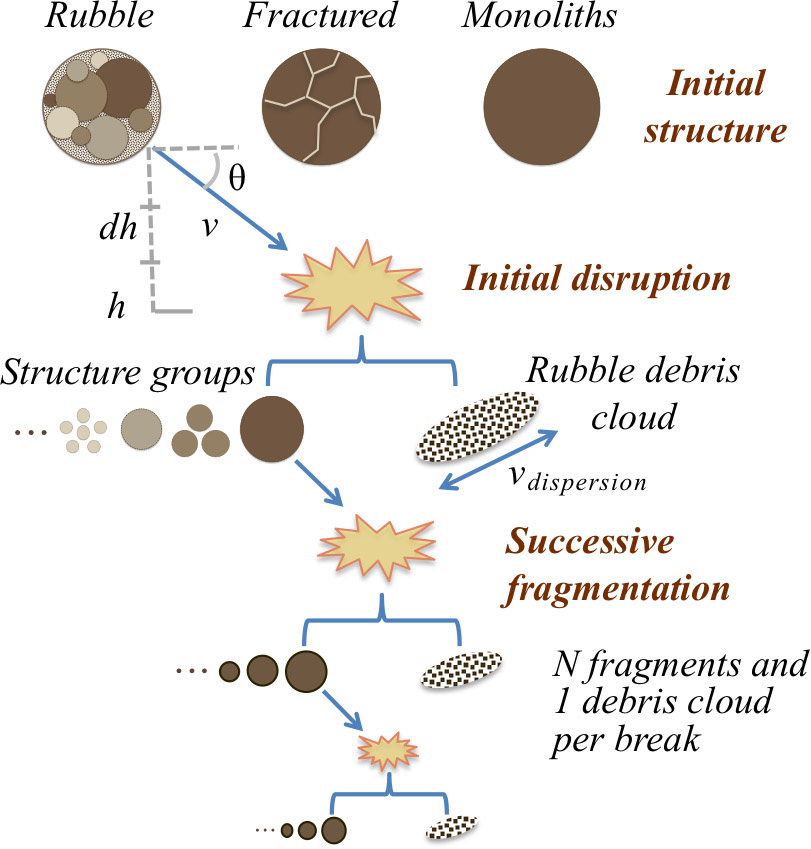
\includegraphics[width=0.7\textwidth]{figures/wheeler_diagram.jpg}
    \caption{FCM model diagram, taken from \cite{wheeler2018atmospheric}.
        A meteoroid is modeled to enter a planetary atmosphere with a speed $v$ and a trajectory angle $\theta$ relative to the ground. When the ram pressure exceeds its aerodynamic strength at height $h$ above the ground, it fragments into different structural groups, and a debris cloud. The debris cloud is described with a ``pancake''-style model. The fragments descend further into the atmosphere and may undergo successive fragmentation when their aerodynamic strength is exceeded.\label{fig:FCMv2}}
\end{figure*}

\subsection{Impact}

Once fragments of the meteoroid impact the ground, we use a well-established scaling relationship to determine the crater diameters $D$ \citep{holsapple1987scaling}.
\begin{align}
    \pi_2 &= \frac{g_0 r}{v_z^2}\,,\quad\pi_3 = \frac{Y}{\rho_t v_z^2}\,,\quad\pi_4 = \frac{\rho_t}{\rho_i}\,, \nonumber \\
    e_1 &= \frac{6\nu - 2 - \mu}{3\mu}\,,\quad e_2 = \frac{6\nu-2}{3\mu} \,, \nonumber \\
    e_3 &= \frac{2+\mu}{2}\,,\quad e_4 = -\frac{3\mu}{2 + \mu} \nonumber \\
    \pi_v &= K_1 \left[\pi_2 \pi_4^{e_1} + K_2 \left(\pi_3 \pi_4^{e_2}\right)^{e_3}\right]^{e_4} \nonumber \\
    V &= \pi_v \frac{m}{\rho_t} \nonumber \\
    D &= 2f_\mathrm{rim} K_r V^{1/3} \label{eq:holsapple2}
\end{align}
This relationship cover a large range of potential surface properties and impact scenarios.
$g_0$ is the gravitational acceleration at the impact location, $r$ the radius of the impacting fragment, $v_z$ its vertical velocity, $m$ its mass and $\rho_i$ its density. Without the factor $f_\mathrm{rim}$, these laws calculate the crater diameter at pre-impact surface level.
Some of the crater ejecta typically form a rim around the crater, which is what is visible on satellite images. We therefore multiply the result by $f_\mathrm{rim} \sim 1.3$ to match observations more closely \citep{daubar2020newcrater}. The ground is modeled with the following properties: Density $\rho_t$, strength $Y$, and a number of coefficients $K_1$, $K_2$, $K_r$, $\mu$, $\nu$. While the library allows for arbitrary values to be set, this work used parameters appropriate for a weak granular soil \citep{holsapple1987scaling}, listed in table~\ref{tab:holsapple_coeff}.  

In cases where two or more craters overlap, they are combined into a single crater with a volume equal to the sum of the two crater volumes.

\begin{table}[htbp]
    \centering
    \begin{tabular}{c|c}
        $\rho_t$ & $1.5\,\mathrm{\frac{g}{cm^3}}$ \\
        $Y$ & $50\,\mathrm{kPa}$ \\
        $K_1$ & 0.133 \\
        $K_2$ & 1.0 \\
        $K_r$ & 1.25 \\
        $\mu$ & 0.41 \\
        $\nu$ & 0.40 \\
        $f_\mathrm{rim}$ & 1.3
    \end{tabular}
    \caption{Coefficients used for Holsapple scaling laws (eq.~\ref{eq:holsapple2}).}
    \label{tab:holsapple_coeff}
\end{table}

\subsection{Implementation}
\label{sec:implementation}
The main goal of the implementation was to develop a flexible, high-performance library. The implementation used in a similar work \citep{newland2019CFM18} was available, but was severely limited in performance and scalability. Its main limiting factor was that it was written entirely in Python. It performed well enough to be usable for entirely cloud-driven models, as well as for scenarios with few fragments. However, for meteoroids heavier than a few kilograms, the number of fragments produced by the model can soon reach tens of thousands, which brings the solver to a crawl. Because of the iterative nature of any ODE solver, the solver loop cannot be vectorised.
We therefore re-implemented the forward model in a compiled language, C++.
For ease of use, we developed a Python API for it, and plan to release the entire library as a Python package.

The library provides multiple ODE solver options for equations \ref{eq:dvdt} - \ref{eq:dydt} and \ref{eq:DCM} - \ref{eq:CRM}.
Contrary to what \cite{wheeler2017fragmentcloud} proposed, our implementation uses a more conventional time stepping scheme, rather than setting a fixed height step size of e.g. $\delta z = 10\unit{m}$.

\subsubsection{Performance optimizations}
The library provides the option to use either a fixed or an adaptive time step size that adjusts to the estimated local error of each fragment and debris cloud individually. It offers second and fourth order accurate schemes. In our convergence analysis, we found that with a variable step size, our model achieves the same accuracy at $1/3$ of the number of iterations compared to a fixed time step size. It avoids wasting computation time early on in the simulation, when not much is happening in the thin upper atmosphere, while significantly decreasing the step size when fragmentation is happening and rapidly ablating/decelerating debris clouds and tiny fragments are formed.

Opting for a time stepping scheme instead of Wheeler et al.'s fixed $z$ step poses two challenges that we had to address. First, any time stepping scheme will overshoot the moment of impact ($z_\mathrm{final} < z_\mathrm{ground}$), which is not the case if the $z$ step size is chosen correctly. The solution is straightforward: we decrease the last step size such that $z_\mathrm{final} = z_\mathrm{ground}$ exactly. Second, in the case of a variable step size, which is different for each fragment in the simulation, calculating the energy deposition in the atmosphere per unit height, $dE/dz$, requires interpolation. As a side note, a similar overshooting problem and the solution that we came up with is described in appendix~\ref{sec:overshoot}. This last problem is also present in the ODE solving approach that \cite{wheeler2017fragmentcloud} used.

Another significant performance advantage of our model is that we exclude fragments from the simulation that are no longer relevant in two ways: First, if a fragment or a debris cloud would produce an impact crater that is smaller than a pre-defined threshold, and second if a debris cloud has deposited practically all its kinetic energy into the atmosphere. Both avoid needlessly tracking tiny fragments that would form craters too small to detect. 
All these techniques combined yield an enormous performance increase; we see between two and three orders of magnitude improvement compared to the Python implementation.
It is now feasible to run Monte-Carlo simulations within minutes instead of hours. Potential use cases of the library are numerous. We utilize it in the following sections to investigate martian crater clusters.


\section{Crater Cluster Characteristics}
\label{sec:characteristics}
A meteoroid in our model is described with a number of features before it starts descending through the atmosphere.
It has a mass, a velocity, a density, a trajectory angle relative to the planetary surface, and a strength that indicates how much aerodynamic stress it can withstand before breaking up into pieces. 

In a survey of 77 recent impact crater clusters on Mars, \cite{daubar2019recently} studied a number of characteristics of these clusters.
In the following work, we investigate whether these characteristics allow us to constrain the range of possible values for the meteoroid features; e.g., whether we can constrain the mass of the meteoroid based on a combination of these characteristics.

Because of the limited scope of this project, we had to make a handful of arbitrary choices about the variant of our model to use.
Our choices were largely based on the work by \cite{newland2019CFM18}. They used the fragment-cloud model (sec.~\ref{sec:fragment_cloud_model}) with random fragment mass fractions, but without the random element to strength scaling (cf. sec.~\ref{sec:fragments_model}).
\cite{newland2019CFM18} also made use of the 2018 extension to the fragment-cloud model that specifies an inner meteoroid structure.
Based on the results presented in \cite{wheeler2018atmospheric}, \cite{newland2019CFM18} defined a simplified inner structure outlined in table~\ref{tab:eric_inner_structure}.
Three structural groups are specified, all making up one third of the total meteoroid mass.
At first break up, the meteoroid will split into 13 pieces, in total, of varying size.
The smaller pieces have a considerably smaller strength $\sigma_b$ compared to the largest piece with a strength of $\sigma_c$. The medium size pieces of the second group are in between.
This reflects the findings by \cite{wheeler2018atmospheric}, who found that in their simulations, best agreement with the data was achieved if, in general, the larger pieces in their inner structure had a higher strength.
Assuming this inner structure, \cite{newland2019CFM18} were able to produce a distribution of certain cluster characteristics that was similar to the clusters presented in the \cite{daubar2019recently} survey. Such a good match to observation was not possible when a homogeneous inner structure was used.
This model is therefore a good starting point for our study.

\begin{table}[htbp]
    \centering
    \begin{tabular}{r|ccc}
        mass fraction (\%) & & $1/3$ \\
        pieces & $1$ & $3$ & $9$ \\
        strength & $\sigma_c$ & $\sqrt{\sigma_c\sigma_b}$ & $\sigma_b$ \\
        Weibull exponent & & $0.25$ \\
        cloud mass fraction & & $0.5$ \\
        frag. mass fractions & \multicolumn{3}{c}{$(0.05 - 0.5$, $0.5 - 0.95)$}
    \end{tabular}
    \caption{Meteoroid inner structure proposed by \cite{newland2019CFM18}, based on results from \cite{wheeler2018atmospheric}. For the Weibull exponent and the cloud mass fraction, we chose a fixed value based on the average used in \cite{wheeler2018atmospheric}.}
    \label{tab:eric_inner_structure}
\end{table}

The characteristics studied by \cite{daubar2019recently} and \cite{newland2019CFM18} are listed in table~\ref{tab:charcteristics}. For each of these, we studied (a) how variable they are for a given meteoroid as a result of randomness in the breakup process, and (b) how well they constrain the range of possible meteoroid features.
For (a), we defined a set of meteoroid features that is representative of the space of possible values.
Then we repeated the same simulation with different seeds to the random number generator (RNG) and computed the crater characteristics. Two examples are displayed in figures \ref{fig:characteristics_variability_1} and \ref{fig:characteristics_variability_2}.
For (b), we ran a Monte-Carlo simulation across the entire range of meteoroid features that would lead to a cluster with effective diameter between about $1\,\mathrm{m}$ and $50\,\mathrm{m}$.
Parameters for both parts are listed in table~\ref{tab:mc_params}.

\begin{figure*}
    \centering
    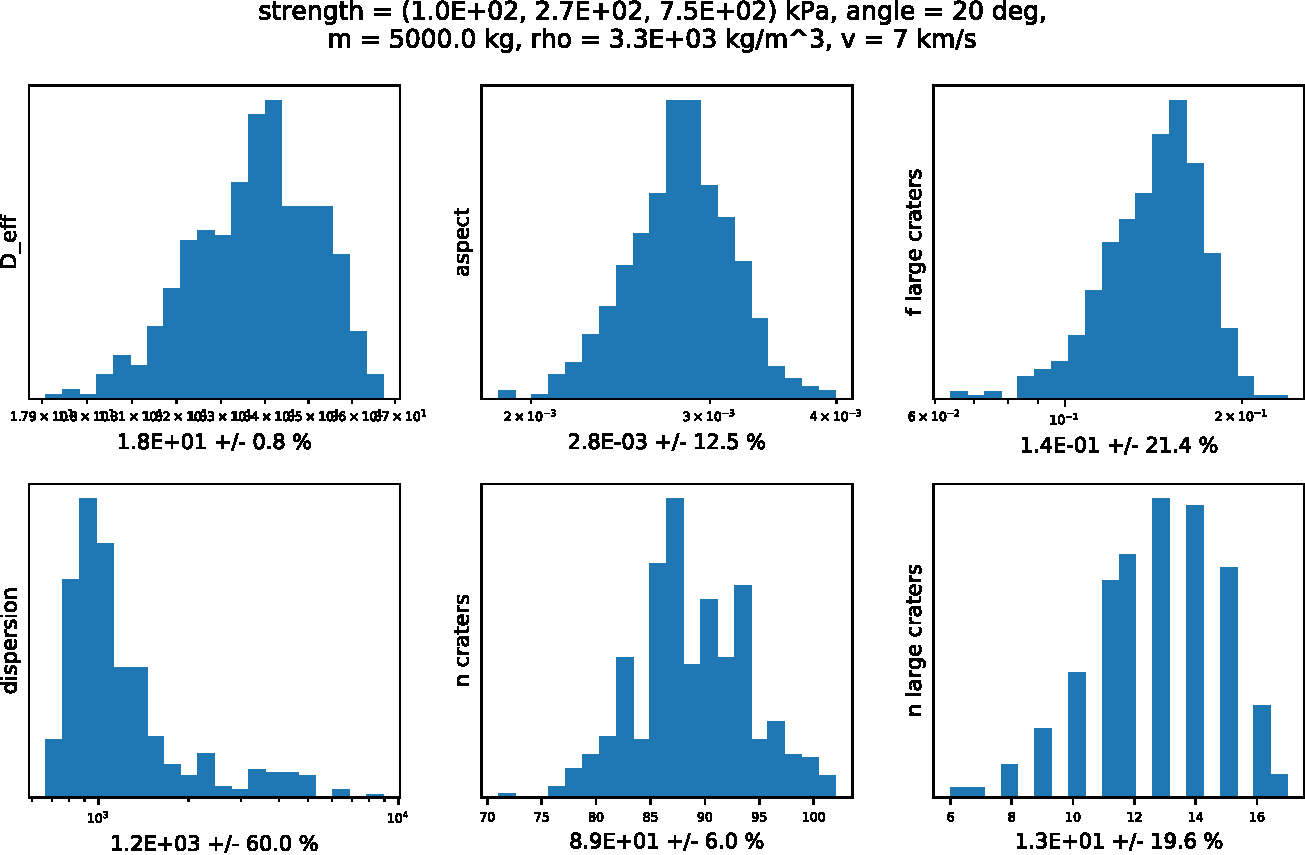
\includegraphics[width=\textwidth]{figures/crater_tools_analysis_1}
    \caption{Crater characteristics computed from running the forward model with parameters in the title and 500 different seeds for the random number generator.}
    \label{fig:characteristics_variability_1}
\end{figure*}

\begin{figure*}
    \centering
    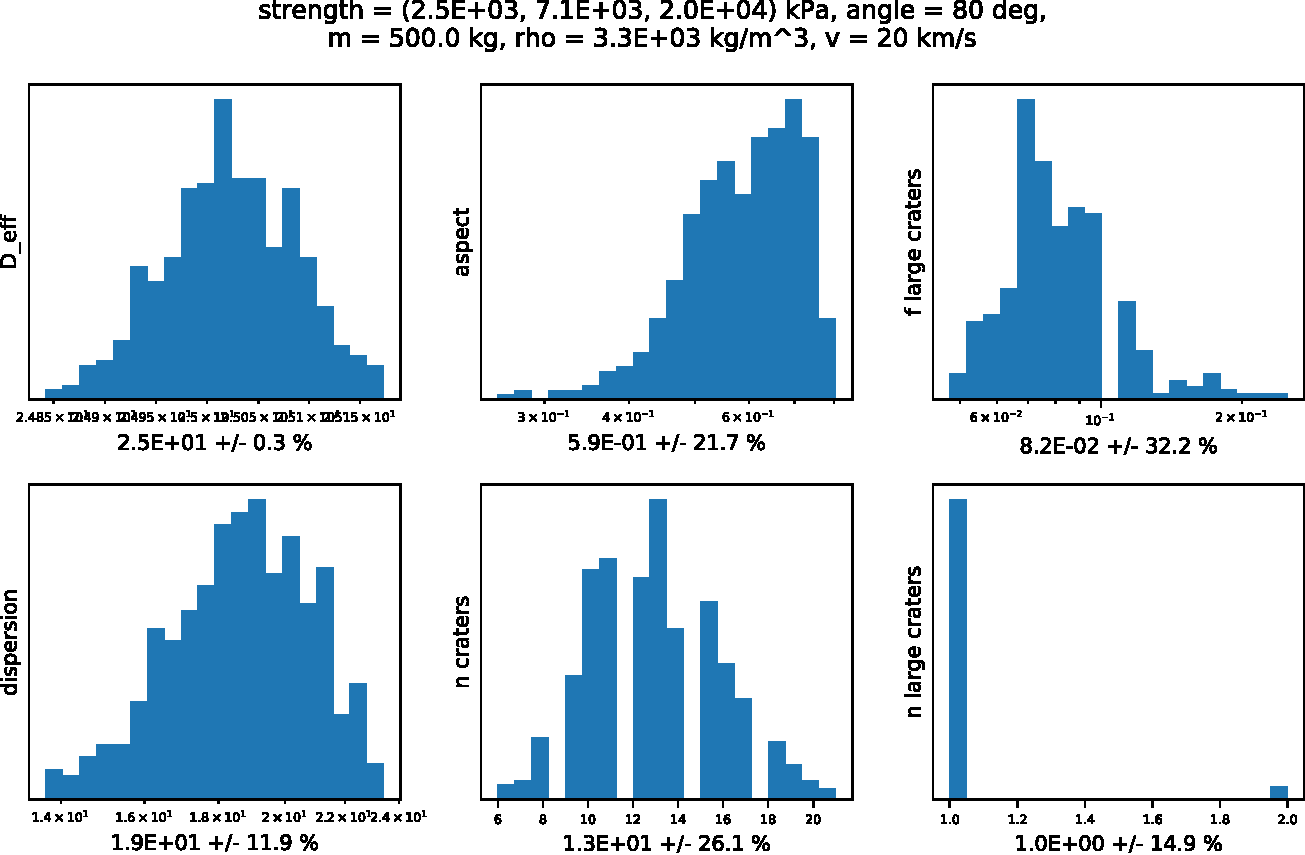
\includegraphics[width=\textwidth]{figures/crater_tools_analysis_2}
    \caption{Crater characteristics computed from running the forward model with the same parameters in the title 500 different seeds for the random number generator.}
    \label{fig:characteristics_variability_2}
\end{figure*}

\begin{table}[htbp]
    \centering
    \begin{tabular}{l|l}
        effective diameter & $\left(\sum_i d_i^3\right)^{1/3}$, $d_i$ the \\ & crater diameters \\[0.4em]
        aspect ratio & ratio of minor to major \\ & axis of best fit ellipse \\ & around the cluster \\[0.4em]
        dispersion & median distance \\ & between craters \\[0.4em]
        $n$ craters & number of craters \\ & in a cluster \\[0.4em]
        $f$ large craters & fraction of craters \\ & larger than a threshold
    \end{tabular}
    \caption{Crater characteristics studied by \cite{daubar2019recently} and/or \cite{newland2019CFM18}.}
    \label{tab:charcteristics}
\end{table}

\begin{table*}
    \centering
    \begin{tabular}{l|l l}
        & \multicolumn{1}{c}{(a)} & \multicolumn{1}{c}{(b)} \\
        \hline
        mass $m$ (kg) & $\log(m) \sim \mathcal{U}[\log(0.1),\, \log(2\e{4})]$ & $m \in \{0.3, 500, 500 \}\unit{kg}$ \\
        density $\rho$ & \multicolumn{2}{c}{$\rho = 3330 \unit{\frac{kg}{m^3}}$} \\
        velocity $v$ (km/s) & $\log(v) \sim \mathcal{U}[\log(6),\, \log(30)]$ & $v \in \{7, 12, 20\} \unit{\frac{km}{s}}$ \\
        bulk strength $\sigma_b$ (kPa) & $\log(\sigma_b) \sim \mathcal{U}[\log(1),\, \log(10^5)]$ & $\sigma_b \in \{100, 500, 2500\} \unit{kPa}$ \\
        core strength $\sigma_c$ (kPa) & $\log(\sigma_c) \sim \mathcal{U}[\log(\sigma_b),\, \log(10^5)]$ & $\sigma_c \in \{750, 4000, 2\e{4}\} \unit{kPa}$ \\
        angle $\theta$ (deg) & $\log(\theta) \sim \mathcal{U}[\log(10),\, \log(90)]$ & $\theta \in \{20, 45, 80\}\unit{deg}$
    \end{tabular}
    \caption{Meteoroid features used for the Monte-Carlo studies in section~\ref{sec:characteristics}. $x\sim\mathcal{U}[a, b]$ means that the value $x$ is drawn from a uniform distribution in the interval $[a, b]$. For $\theta < 10\unit{deg}$, the meteoroid almost always either escaped the atmosphere again in our simulation or did not produce detectable craters.}
    \label{tab:mc_params}
\end{table*}

\subsection{Effective diameter}
The effective diameter $D_\mathrm{eff}$ of a crater cluster is a measure of the total volume of all craters. A common assumption is that it is a good proxy for the impactor mass (citation needed).
Figure~\ref{fig:d_eff_vs_m} shows that the relationship is a bit more complicated. We can infer that for our model, $D_\mathrm{eff}$ provides a lower bound for the meteoroid mass, but that the spread of meteoroid masses that can produce clusters of the same $D_\mathrm{eff}$ is quite wide.
Fig.~\ref{fig:d_eff_vs_m} is colour coded by the trajectory angle $\theta$. It shows that a shallower angle increases the lower bound for the mass significantly.
At a given angle, most samples are within a band close to the lower bound, except for a number of outliers. The outliers mostly occur for weak meteoroids.

\begin{figure*}
    \centering
    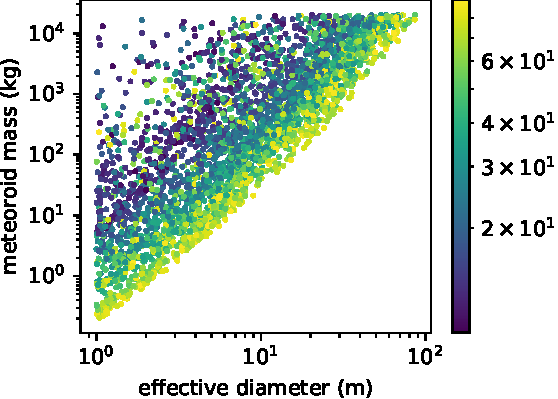
\includegraphics[width=0.45\textwidth]{figures/d_eff_vs_mass}
    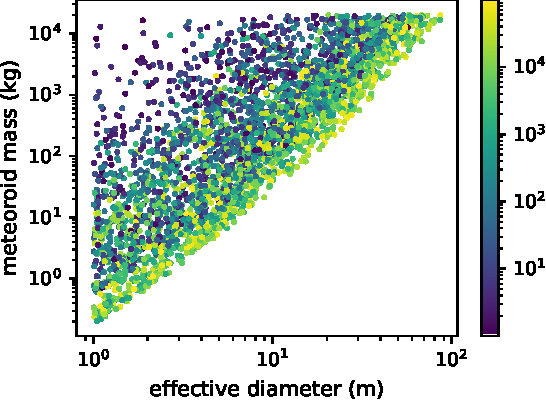
\includegraphics[width=0.45\textwidth]{figures/d_eff_vs_mass_strength}
    \caption{Effective diameter vs initial meteoroid mass. Left colour = initial trajectory angle in degrees from horizontal. Right colour = core strength $\sigma_c$. We can see that at a given angle, mass and effective diameter are highly correlated. Similarly for a given strength.}
    \label{fig:d_eff_vs_m}
\end{figure*}

$D_\mathrm{eff}$ also provides useful information about the strength of the largest piece ($\sigma_c$ in tab.~\ref{tab:eric_inner_structure}) in our inner structure. Figure~\ref{fig:d_eff_vs_strength} shows that at a given meteoroid mass, there is an upper limit to the effective diameter that the cluster can have, and that this limit increases for higher core strengths.
The same pattern cannot be observed for the strengths of the other structural groups. This is probably because the effective diameter is dominated by the largest craters produced by the largest pieces, which will be produced by fragments of the strongest group.

\begin{figure*}
    \centering
    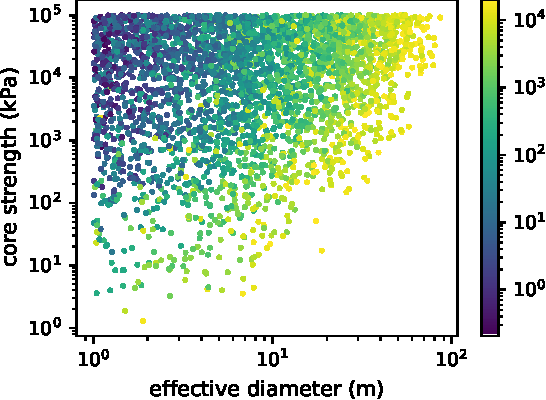
\includegraphics[width=0.7\textwidth]{figures/d_eff_vs_strength}
    \caption{Effective diameter vs. core strength ($\sigma_c$ in tab.~\ref{tab:eric_inner_structure}). The colour code corresponds to the meteoroid mass in kg. We can see that at a given mass, $\sigma_c$ and effective diameter are correlated.}
    \label{fig:d_eff_vs_strength}
\end{figure*}

Overall, we conclude that $D_\mathrm{eff}$ provides useful information about the meteoroid mass and strength, and constrains the most likely values even better if other measures are taken into account that restrict the trajectory angle and meteoroid strength. The analysis with variable RNG seeds shows that it is by far the most stable characteristic out of the ones we considered. The relative variability is of the order of $1 - 2\%$ in all scenarios that we looked at.

\subsection{Aspect ratio}
The aspect ratio is defined as the ratio of the semi-minor and semi-major axis of the ellipse with the smallest area that envelops all craters in a cluster.
It was proposed in the \cite{daubar2019recently} survey as a proxy for the initial trajectory angle $\theta$. 
There are several ways to compute this ratio. In this study, we use principal component analysis (PCA).
The ratio of variances explained by the two principal components is equal to the aspect ratio. In order to limit the influence of outlier craters, we average the result over a number of bootstrapped samples. An example of a best-fit ellipse around a crater cluster can be seen in fig.~\ref{fig:ellipse_example}.

\begin{figure*}
    \centering
    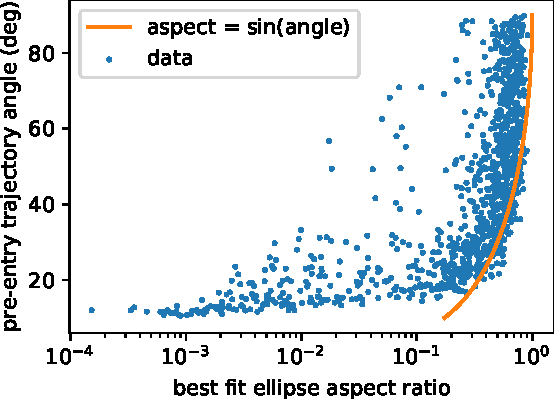
\includegraphics[width=0.7\textwidth]{figures/aspect_vs_angle}
    \caption{Aspect ratio vs initial trajectory angle. The orange line indicates the relationship proposed in \cite{daubar2019recently}.}
    \label{fig:aspect_vs_angle}
\end{figure*}

Figure~\ref{fig:aspect_vs_angle} shows the connection between the two. We can see that, similar to what was proposed in \cite{daubar2019recently}, the dispersion is almost independent of $\theta$ for angles above $\sim$40 degrees.
For shallower angles however, the angle dominates other meteoroid features. This behaviour is what we would expect qualitatively; at steep angles, we expect the spatial distribution of craters to be dominated by random processes during the breakup events.
Indeed, our analysis shows that varying the RNG seed introduces relative variances of typically $~30\%$ if the other parameters are kept at a constant value.

\subsection{Dispersion}
The dispersion attempts to measure the total size of a cluster as seen on the photos.
A first idea for a measure might be the maximum distance between any two craters in a cluster.
Since this measure would be prone to outliers, \cite{daubar2019recently} suggested to instead consider the entire set of distances between all pairs of craters.
They then calculated the standard deviation of this set of distances.
In this work, we use the median distance. We found that it is often very similar to the standard deviation. Plus, it can also be defined for clusters with only two craters.

In our variable RNG seed analysis, we see that the dispersion is quite well defined for the two steeper trajectory angles (45 and 80 degrees). The relative error is between 10 - 15\%. At shallower angles, dispersion becomes significantly more variable with relative errors of $\sim$50\%. 

\begin{figure*}
    \centering
    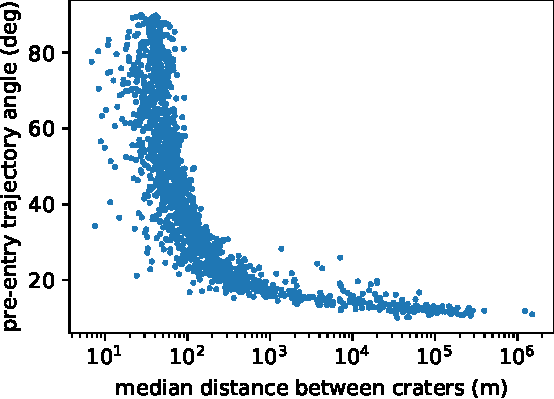
\includegraphics[width=0.7\textwidth]{figures/disp_vs_angle}
    \caption{Median dispersion vs. initial trajectory angle.}
    \label{fig:disp_vs_angle}
\end{figure*}

For high values of dispersion, Figure~\ref{fig:disp_vs_angle} shows that in our model, the dispersion is largely influenced by the pre-entry impact angle. In fact, as figure~\ref{fig:disp_vs_aspect} shows, an important limitation of our model is that high levels of dispersion only occur for smaller aspect ratios.

Only considering one measure of the distribution of separation distances has its limitations however. In future work, we might want to consider additional features of this distribution. For example, the median or standard deviation does not capture sub-clustering of craters; that is, pockets of nearby craters that are clearly separated from the others.

\begin{figure*}
    \centering
    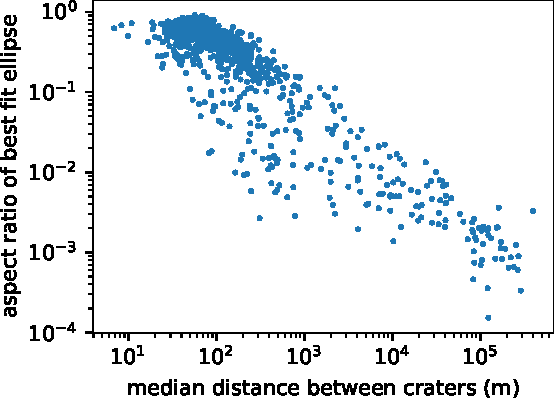
\includegraphics[width=0.7\textwidth]{figures/disp_vs_aspect}
    \caption{Median dispersion vs. aspect ratio of best-fit ellipse. It shows that there is a threshold for dispersion above which our model can only produce clusters with that value if they are distributed within a tight ellipse. For the model parameters we used, the threshold is about $100\unit{m}$.}
    \label{fig:disp_vs_aspect}
\end{figure*}

\subsection{Number of craters}
The crater clusters mapped by \cite{daubar2019recently} only contain craters with a diameter of at least $1\unit{m}$, which is linked to the resolution of the images that they worked with.
Because of this limit, we would expect the number of craters large enough to be visible to provide a lower limit to the effective diameter, and therefore to the mass of the impactor, which is indeed what Fig.~\ref{fig:n_craters_vs_m} shows for clusters of more than 20 craters.
The number of craters generally varies by about 15 - 20\%.

\begin{figure*}
    \centering
    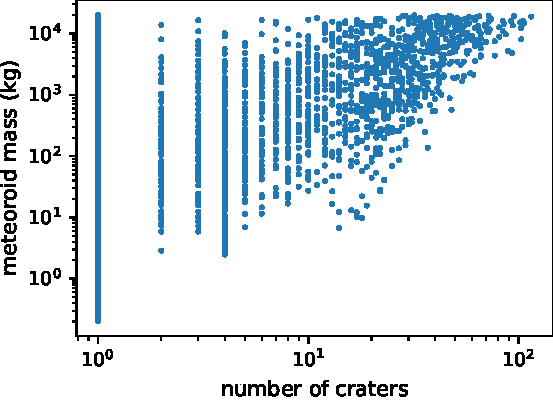
\includegraphics[width=0.7\textwidth]{figures/n_craters_vs_mass}
    \caption{Number of craters vs. initial meteoroid mass. Above about 20 craters, it provides a lower limit to the meteoroid mass. There is also a minimum mass to form at least two detectable craters.}
    \label{fig:n_craters_vs_m}
\end{figure*}

\subsection{Fraction of large craters}
Considering this measure was proposed by \cite{newland2019CFM18}, who attempted to find a way to quantify the diameter-frequency distribution of craters in the clusters. The definition of a large crater is that its diameter $d_i$ has to be larger than a fraction $f$ of the largest diameter $d_\mathrm{max}$.
\begin{equation}
    f_\mathrm{large\,craters} = \left|\left\{d_i\ \big|\ d_i > f\cdot d_\mathrm{max}\right\}\right|
\end{equation}
\cite{newland2019CFM18} used $f = 0.5$ and were able to show that, with the inner structure in Table~\ref{tab:eric_inner_structure}, the fraction of large craters produced by the fragment-cloud model, at a given effective diameter, exhibits a similar distribution to the observational data \citep{daubar2019recently}. If they assumed a homogeneous inner structure however, this was decidedly not the case. It allowed them therefore to make a claim about the general inner structure of impactors on Mars.

In this work, we kept the inner structure fixed. We did not see an appreciable influence that fixing this quantity had on any of the meteoroid features.
Aside from an obvious one, where there is a minimum mass required to get a very small fraction of large craters (cf. fig.~\ref{fig:f_large_vs_mass}). This is what we would expect if there are one or two large craters; in order to form a sufficiently large number of small craters, a larger mass is required (Figure~\ref{fig:n_craters_vs_m}).

\begin{figure*}
    \centering
    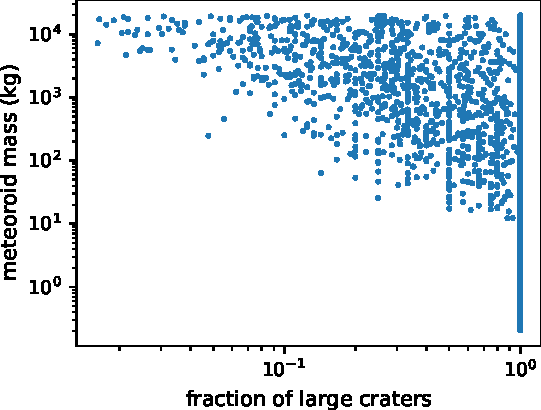
\includegraphics[width=0.7\textwidth]{figures/f_large_vs_mass}
    \caption{Number of craters vs. initial meteoroid mass. Above about 20 craters, it provides a lower limit to the meteoroid mass. There is also a minimum mass to form at least two detectable craters.}
    \label{fig:f_large_vs_mass}
\end{figure*}

\subsection{Summary}

Table~\ref{tab:characteristics_summary} contains an overview of the findings presented above. We were able to show that there is no simple relationship by which meteoroid feature determines any characteristic of the crater cluster that it forms. We have identified two reasons for this. Even though many of these characteristics are defined in a way that should be rather resilient to outliers, our simulations show randomness in the breakup events of our model leads to significant variability.

Second, our Monte-Carlo simulation shows that a whole range of parameters can result in the same effective diameter for example.
But we have also found limits to this range of parameters. Only a limited range of combinations of mass, angle and core strength produce a similar number of craters and a similar effective diameter. For the dispersion and ellipse aspect ratio, both appear to be suitable indicators for impact angles shallower than 40 degrees.

It should therefore be possible to compute a distribution of meteoroid features that should be reasonably constrained in all features but velocity, which is what we investigate in the next section.

\begin{table*}
    \centering
    \begin{tabular}{l|c|c}
        & relative std deviation & significant parameters \\
        \hline
        $D_\mathrm{eff}$ & $\sim 1\%$ & mass, core strength, angle \\
        aspect & $\sim 30\%$ & angle \\
        dispersion & $\sim 10\%$ (steep $\theta$) - $\sim 60\%$ (shallow $\theta$) & angle \\
        $n$ craters & $ \sim 20\%$ & mass \\
        $f$ large craters & $\sim 30\%$& inner structure \citep{newland2019CFM18}, mass
    \end{tabular}
    \caption{Summary of findings on cluster characteristics}
    \label{tab:characteristics_summary}
\end{table*}


\section{Inversion}
\label{sec:inversion}
A standard technique for inversion of probabilistic forward models is Markov chain Monte Carlo (MCMC) \citep[e.g.,][]{gelfand1990sampling}. The algorithms developed for this technique perform a random walk in the parameter space $\mathcal{P}$ that approaches the posterior distribution defined by Bayes' theorem 
\begin{equation}
    p(A|B) \propto p(A)p(B|A)\,.
\end{equation}
In our case, $A \in \mathcal{P}$ are the meteoroid parameters (mass, velocity, trajectory angle, density, inner structure), and $B|A$ are the characteristics of the crater cluster (effective diameter, dispersion, \dots) produced by our model with input parameters $A$.
Given an image of a real cluster of impact craters, we determine its characteristics $B$. Together with the knowledge from the previous section about the variability of these characteristics, we can compute the likelihood $p(B|A)$ that our model, with parameters $A$, produces a cluster with the same characteristics $B$ as the real image.
With Bayes' theorem, we can infer the likelihood of parameters $A$ given the observation $B$. $p(A)$ expresses any prior knowledge about the input parameters.

A number of MCMC algorithms are available. 
We opted for a rather simple one, that is the Metropolis-Hastings algorithm \citep{10.1093/biomet/57.1.97} with Metropolis sampling.
The latter assumes that there is no correlation between the different model parameters, which as far as we know is a valid assumption.
The Metropolis-Hastings algorithm performs a random walk in the parameter space $(A_i) \in \mathcal{P}$.
The step $A_{i+1} - A_i$ is determined by the Metropolis sampler, which draws samples from a multivariate Gaussian distribution. $A_{i+1}$ is accepted if
\begin{equation}
    \frac{p(A_{i+1}) p(B|A_{i+1})}{p(A_{i}) p(B|A_{i})} > x\,,\quad x \sim \mathcal{U}[0, 1]
\end{equation}

\subsection{Implementation}

From observations, the prior distributions of mass \citep{bland2006rate}, velocity \citep{lefeuvre2011nonuniform} and density \citep{Zijans_source} are known quite well.
For the trajectory angle, we made a simple analysis outlined in Appendix~\ref{sec:angle_prior}. Not much is known about the aerodynamic strength. Meteorites collected on Earth show a maximum strength of 330 MPa \cite{popova2013chelyabinsk}. Having survived atmospheric entry, these samples are certainly not representative of the actual distribution. For this study we decided to assume a flat distribution in log space.

Mass, angle and strength are sampled in log space, velocity and density in linear space. Sampling the angle in log space makes the step size smaller for shallower angles, which we thought was desirable based on the results from section~\ref{sec:characteristics}.
Our Metropolis sampler uses covariance matrix tuning to achieve a target acceptance ratio. At regular intervals, the values of the matrix are adjusted based on the accepted samples and the acceptance ratio in the previous interval.

Based on the results from section~\ref{sec:characteristics}, we defined the likelihood $p(B|A)$ to be the product of likelihoods for all 5 characteristics. We assumed that all characteristics are log-normally distributed with the standard deviations observed in our variable seed simulations (Table~\ref{tab:characteristics_summary}).

The ratio of accepted vs. rejected samples is called the acceptance ratio.
Because MCMC algorithms reach the desired distribution only asymptotically, the first $n$ samples have to be discarded, which is called the burn-in phase.
During burn-in, the goal is to find the region in $\mathcal{P}$ of maximum likelihood.
Therefore, we set the target acceptance ratio in this phase to 20\% to avoid getting stuck in a local minimum or not converging at all.
When the region of maximum likelihood is reached, the target is raised to 50\% to speed up sampling.

\subsection{Results}

We did not get past a proof-of-concept stage for this part of the study, so we are only able to report on preliminary results.
The algorithm is often not quite able to find a region in the parameter space that satisfies all crater characteristics. But it is not far off.
The desired effective diameter can always be reached. The total number of craters is most often a bit too large, as is the total number of large craters.

With the value of $3C/2 = 0.19$ in Equation~\ref{eq:v_t} \citep{artemieva2001motion}, the algorithm is not able to find a combination of input parameters that lead to the desired dispersion and aspect ratio in most cases. The impact angle often has to be very shallow to produce results with a high enough dispersion, which makes the aspect ratio much smaller than desired. A value of 
$C\sim 1$, as originally proposed by \cite{passey1980effects}, alleviates this problem for the most part.

An example of a posterior distribution is given in figures \ref{fig:inversion_example_1} and \ref{fig:inversion_example_2}. Looking at all the simulations we did, we often see the mass being fairly well constrained, as well as the impact angle and the meteoroid strength. The pre-entry velocity often tends towards rather high values. We do not have enough knowledge at this point to make a judgement about whether these observations are the result of the model or the inversion algorithm that we are using. This could be subject of further study.

\begin{figure*}
    \centering
    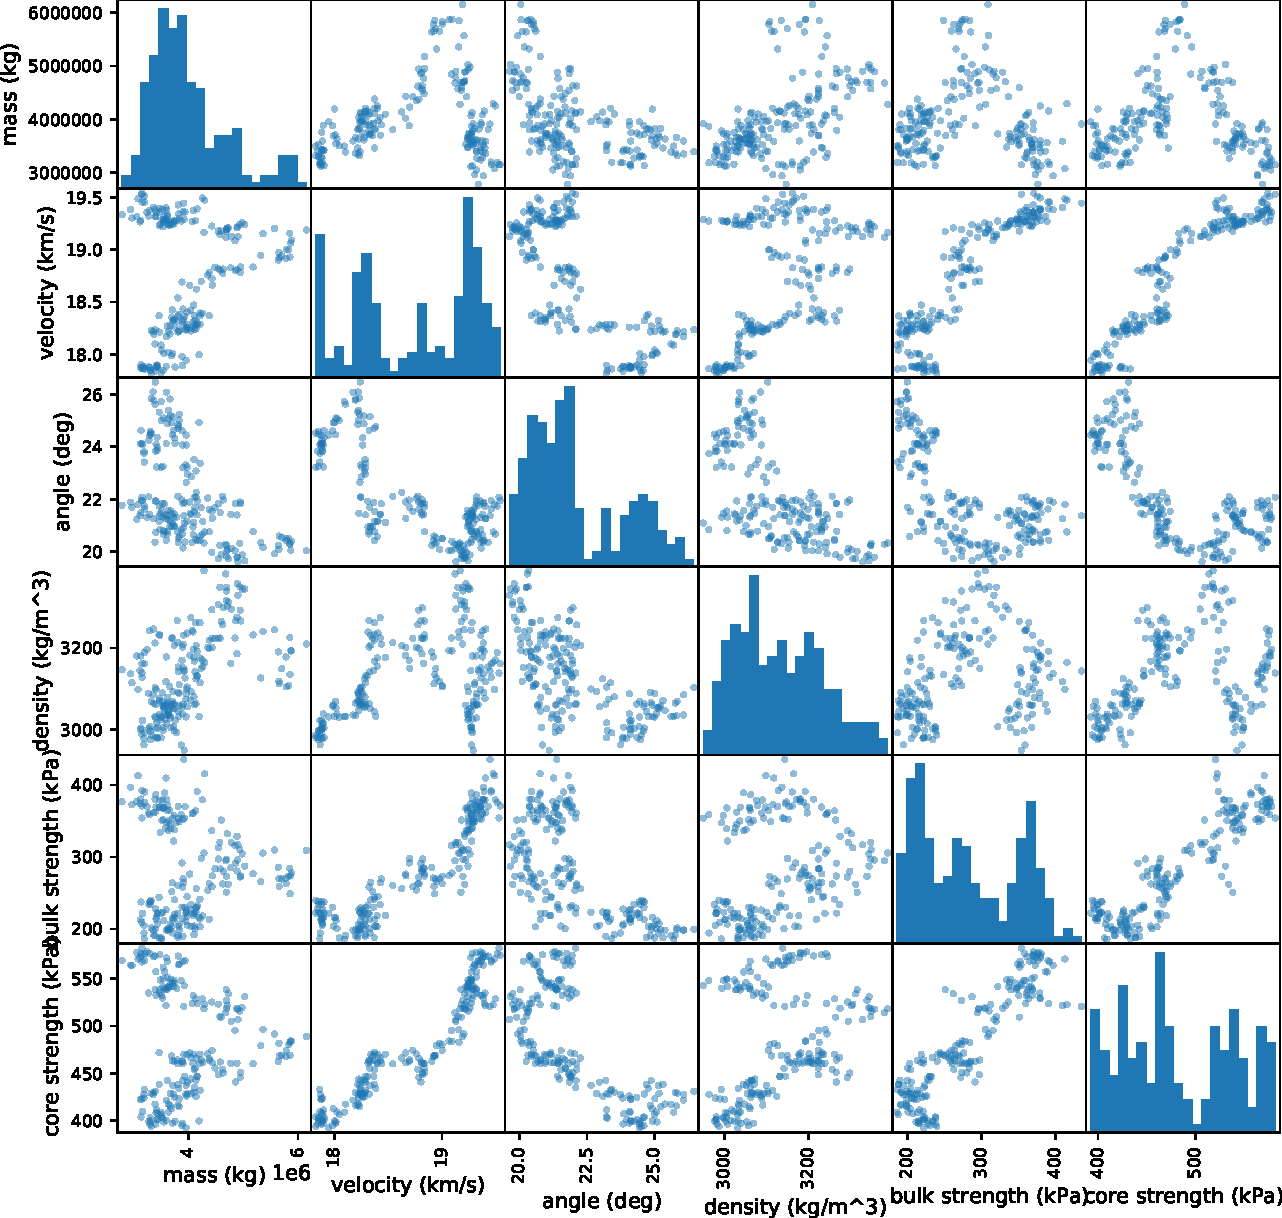
\includegraphics[width=\textwidth]{figures/posterior_ESP_038458_2030}
    \caption{Posterior distribution generated by our inversion algorithm from the observation with HiRISE ID ESP 038458 2030. We can see that the algorithm has not converged yet.}
    \label{fig:inversion_example_1}
\end{figure*}

\begin{figure*}
    \centering
    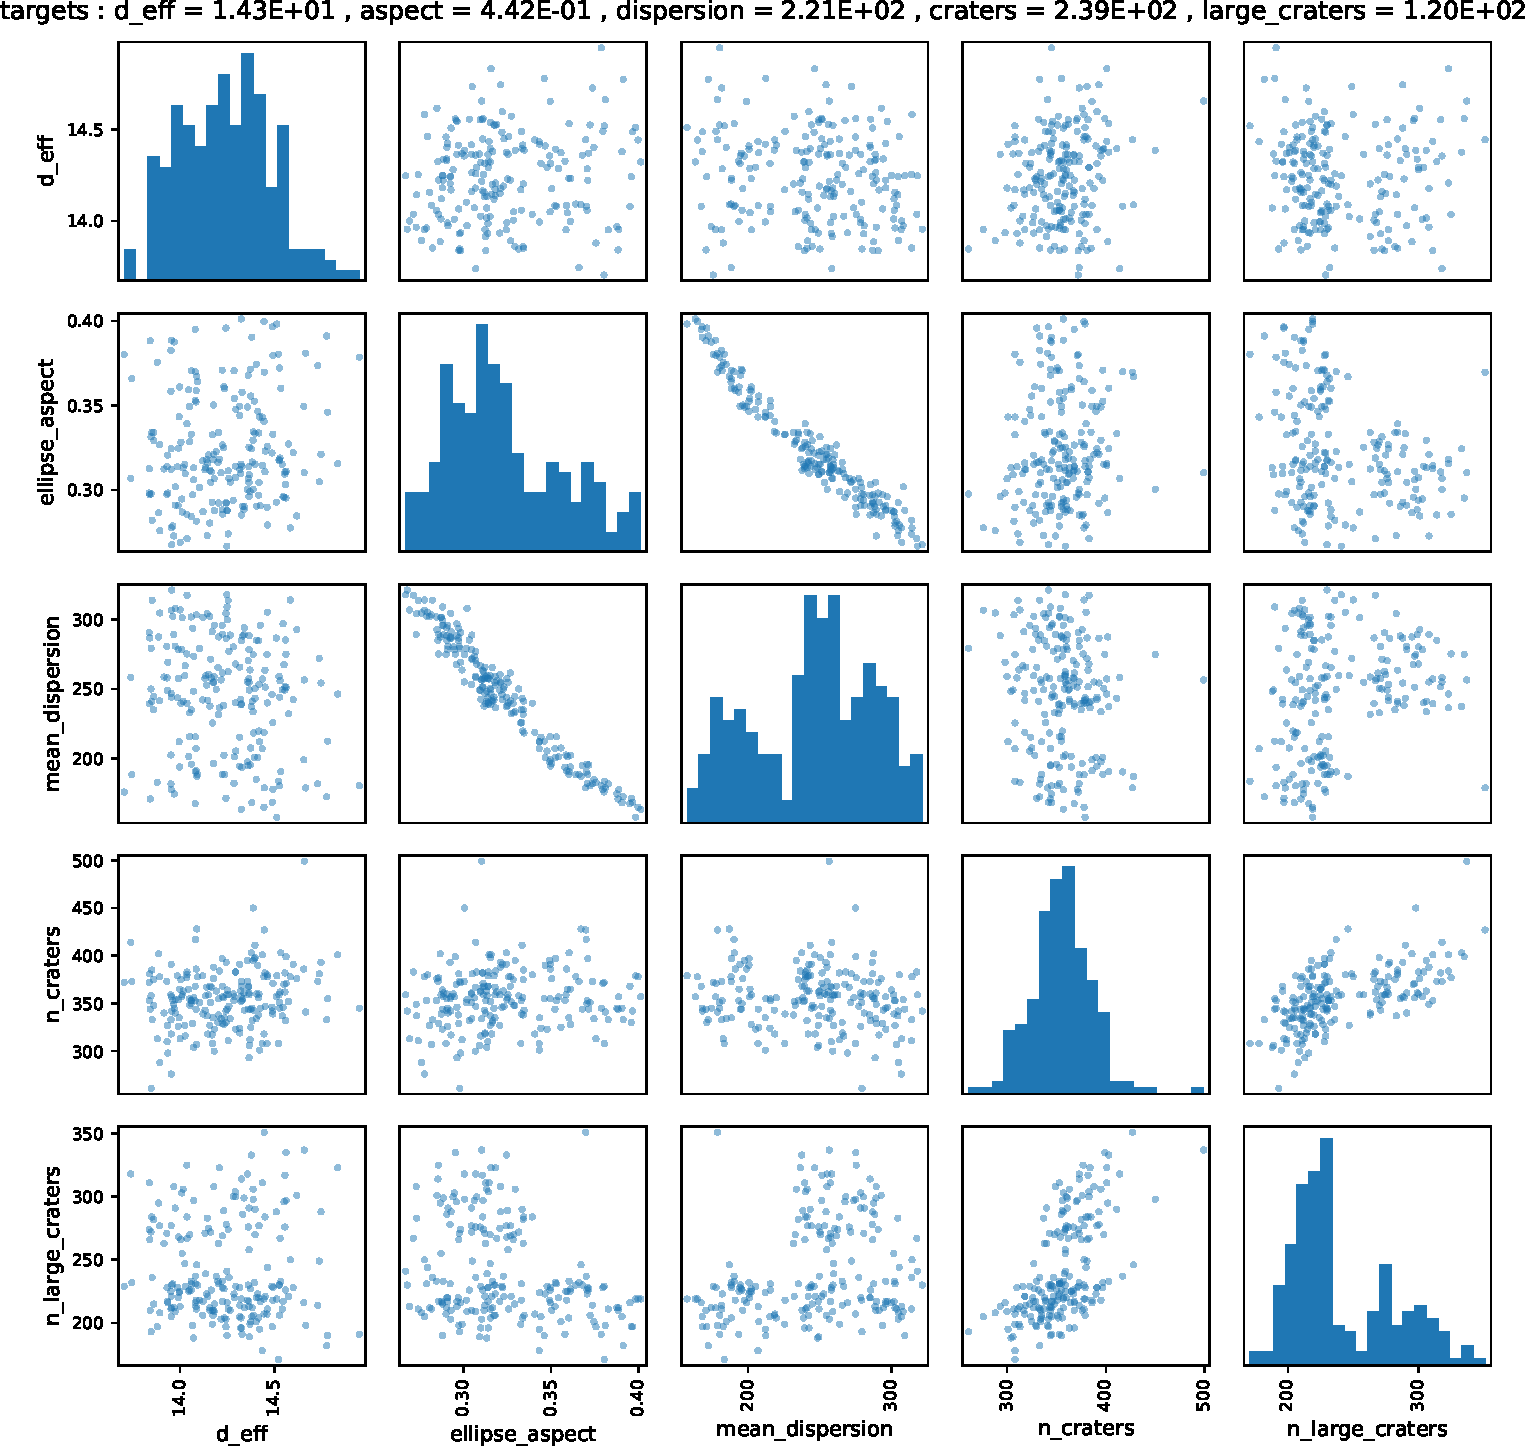
\includegraphics[width=\textwidth]{figures/characteristics_ESP_038458_2030}
    \caption{Cluster characteristics from the posterior distribution in fig.~\ref{fig:inversion_example_1}.}
    \label{fig:inversion_example_2}
\end{figure*}

\section{Discussion}
\label{sec:discussion}
The most useful part of this project probably is the high-performance forward model. It is able to solve atmospheric meteoroid entry with variety of analytical models.
Since it is not bound to our particular use case, it can serve as a foundation for a variety of research projects in the field of atmospheric meteoroid entry.

Our investigation into using inversion techniques to infer meteoroid features like mass or velocity from an image of an impact crater cluster needs a lot more work though. We were able to show that some of the characteristics that \cite{daubar2019recently} and \cite{newland2019CFM18} proposed meaningfully restricted the range of possible features, and that it is feasible to apply an MCMC method for inversion. However, at the current stage of our knowledge, we are not able to properly interpret the results.

Further work could be to investigate what impact a single meteoroid feature like mass has on the characteristics. We might also look into refining the cluster characteristics to extract more meaningful information, particularly out of the distribution of crater diameters in a cluster, as well as the spatial distribution. Both of which are currently condensed into a single number where a lot of information is lost. And finally, in this work we did not at all look into the influence of varying the meteoroid's inner structure, since we assumed that the one proposed by \cite{newland2019CFM18} was representative enough. Further work on the inversion algorithm side might also be necessary to ensure that it samples the entire posterior distribution.


%%% Bibliography %%%
\FloatBarrier

\bibliography{sources}

\clearpage
}

%%% Appendix %%%

\onecolumn{
    \appendix
    \section*{Appendices}
    \subsection{Avoiding overshooting the break up moment}

In our model, we assume that a meteoroid fragments when its aerodynamic strength $\sigma$ is exceeded by the difference in air pressure between opposing sides. The biggest pressure differential will be between the leading edge and trailing edge. The pressure at the leading edge, behind the bow shock, is called the stagnation pressure. The pressure on the other end, in the meteoroid wake, is nearly zero \citep{passey1980effects}. Therefore break up will occur when
\begin{equation}
    \rho_a v^2 = \sigma\,,
\end{equation}
where $\rho_a$ is the air pressure, and $v$ is the meteoroid velocity. Now, in the implementation, the breakup process is triggered when $\rho_a v^2 \geq \sigma$ for the first time. Depending on the time step size used, the overshoot $\rho_a v^2 - \sigma$ might be significant. So here we derive a way to back-track part of the last iteration.

Let $\pmb{p}(t_k) = \pmb{p}_k = (v_k, z_k, m_k, \dots)$ be the current state after $k$ iterations, and $\pmb{p}_{k-1}$ the previous one. Assume $\rho_a(z_k)v_k^2 > \sigma$, and $\rho_a(z_{k-1})v_{k-1}^2 < \sigma$. In essence, we will try to find $\Delta v$ and $\Delta z$ such that
\begin{equation*}
    \rho_a(z_k + \Delta z)\left(v_k + \Delta v\right)^2 = \sigma\,.
\end{equation*}
First, recall that we approximate the air density as follows:
\begin{equation*}
    \rho_a(z) = \rho_0 e^{-z/H}
\end{equation*}
for some scale height $H$, which is itself a function of $z$. It's safe to assume however that $\Delta z$ is small enough that $H(z_k) = H(z_k + \Delta z)$, and $\Delta z \ll H(z_k)$. Therefore,
\begin{equation*}
    \rho_a(z_k + \Delta z) = \rho_0 \exp\left(-\frac{z_k+\Delta z}{H}\right) = \rho_a(z_k)e^{-\Delta z / H}
\end{equation*}
Now, since $\Delta z \ll H(z_k)$, we can use the Taylor approximation:
\begin{align*}
    e^\alpha &= 1 + \alpha + \mathcal{O}(\alpha^2) \\
    \Rightarrow\ \rho_a(z_k + \Delta z) &= \rho_a(z_k)\left(1 - \frac{\Delta z}{H} + \mathcal{O}\left[\left(\frac{\Delta z}{H}\right)^2\right]\right)
\end{align*}
Second,
\begin{equation*}
    (v_k + \Delta v)^2 = v_k^2 + 2v_k\Delta v + \Delta v^2\,.
\end{equation*}
Now, in order to find a relationship between $\Delta z$ and $\Delta v$, recall that
\begin{equation*}
     \frac{dz}{dt} = -\sin(\theta) v\ \Rightarrow\ \Delta z = -\sin(\theta_k) v_k\Delta t\,.
\end{equation*}
Now $\Delta t= \frac{\Delta v}{v_k - v_{k-1}}(t_k - t_{k-1})$
\begin{equation*}
    \Rightarrow\ \Delta z = -v_k\sin(\theta_k)\Delta v\frac{t_k - t_{k-1}}{v_k - v_{k-1}}
\end{equation*}
Putting it all together, we get:
\begin{align*}
    \sigma &= \rho_a(z_k + \Delta z)\left(v_k + \Delta v\right)^2 \\
    &= \rho_a(z_k)\left(1 + \frac{v_k\sin(\theta)\Delta v}{H}\frac{t_k - t_{k-1}}{v_k - v_{k-1}} + \mathcal{O}(\Delta v^2)\right)(v_k^2 + 2v_k\Delta v + \mathcal{O}(\Delta v^2)) \\
    &= \rho_a(z_k)v_k^2 + 2\rho_a(z_k)v_k\Delta v + \rho_a(z_k)v_k^2 \frac{v_k\sin(\theta)\Delta v}{H}\frac{t_k - t_{k-1}}{v_k - v_{k-1}} + \mathcal{O}(\Delta v^2)
\end{align*}
Let $\mathrm{rp} := \rho_a(z_k)v_k^2$. Then
\begin{align*}
    \sigma &= \mathrm{rp} + 2\mathrm{rp}\frac{\Delta v}{v_k} + \mathrm{rp}\frac{v_k\sin(\theta)\Delta v}{H}\frac{t_k - t_{k-1}}{v_k - v_{k-1}} \\
    \Rightarrow\ \frac{\sigma - \mathrm{rp}}{\mathrm{rp}} &= \Delta v \left(\frac{2}{v_k} + \frac{v_k\sin(\theta_k)}{H}\frac{t_k - t_{k-1}}{v_k - v_{k-1}}\right)
\end{align*}
With this expression for $\Delta v$, we can revert back part of the last iteration. We repeat this process until the difference between $\mathrm{rp}$ and $\sigma$ is within our tolerance. In the code specifically, the expression for $\Delta t$ is used:
\begin{align}
    \Delta t &= \Delta v \frac{t_k - t_{k-1}}{v_k - v_{k-1}} \nonumber \\
    &= \left(\frac{\sigma}{\mathrm{rp}} - 1\right) \left(\frac{2}{v_k}\frac{v_k - v_{k-1}}{t_k - t_{k-1}} + \frac{v_k\sin(\theta_k)}{H}\right)^{-1}
\end{align}

\subsection{Fragmentation}

In our model, we adopt the separate fragments approach first proposed by \cite{passey1980effects}.
They derived that after fragmentation, when both the rest of the bolide and the new fragment are traveling under separate bow shocks, 
the fragment will have an additional transverse velocity $V_T$ perpendicular to the bolide trajectory before fragmentation.
Under the assumption that both the fragment and the bolide are spherical objects,
they derived that
\begin{equation}
    V_T = \sqrt{\frac{3}{2}C\frac{R_b}{R_f}\frac{\rho_a}{\rho_f}}V_i\,,
    \label{eq:v_t}
\end{equation}
where $C$ is a dimensionless factor, $R_b$ is the radius of the remaining bolide after fragmentation,
$R_f$ is the radius of the new fragment, $\rho_a$ is the air density, $\rho_f$ is the density of the new fragment,
and $V_i$ is the velocity of the bolide just before fragmentation. $C$ indicates the distance $d = C\cdot R_b$ at which the interaction between the two bow shocks stops.

In our model, we assign a random direction to $V_T$ in the plane perpendicular to the current bolide trajectory.
In order to adhere to momentum conservation, velocities
\begin{align}
    V_T^f &= \frac{m_b}{m_b + m_f}V_T \\
    V_T^b &= \frac{m_f}{m_b + m_f}V_T
    \label{eq:v_t_star}
\end{align}
are added to the two bodies in opposing directions.
$m_f$ and $m_b$ are the new fragment mass and the remaining bolide mass respectively.

In order to add $V_T^f$ and $V_T^b$ to the velocity $\pmb{v}$ that the bolide had just before fragmentation,
we have to calculate its components in our coordinate system.
Recall that in Euclidean coordinates, we have defined
\begin{equation*}
    \pmb{v} = v \begin{pmatrix}
        \cos(\theta)\cos(\phi) \\
        \cos(\theta)\sin(\phi) \\
        -\sin(\theta)
    \end{pmatrix}.
\end{equation*}
We define $\pmb{e}_1 = \frac{\pmb{v}}{v}$.
In order to get an orthonormal basis of the plane perpendicular to $\pmb{v}$, we first rotate $\pmb{e}_1$ by $\frac{\pi}{2}$:
\begin{equation*}
    \pmb{e}_2 = \begin{pmatrix}
        \cos\left(\theta - \frac{\pi}{2}\right)\cos(\phi) \\
        \cos\left(\theta - \frac{\pi}{2}\right)\sin(\phi) \\
        -\sin\left(\theta - \frac{\pi}{2}\right)
    \end{pmatrix} = \begin{pmatrix}
        \sin(\theta)\cos(\phi) \\
        \sin(\theta)\sin(\phi) \\
        \cos(\theta)
    \end{pmatrix}
\end{equation*}
Finally, we calculate the cross product
\begin{align*}
    \pmb{e}_3 &= \pmb{e}_1 \times \pmb{e}_2 \\
    &= \begin{pmatrix}
        \cos(\theta)\cos(\phi) \\
        \cos(\theta)\sin(\phi) \\
        -\sin(\theta)
    \end{pmatrix} \times \begin{pmatrix}
        \sin(\theta)\cos(\phi) \\
        \sin(\theta)\sin(\phi) \\
        \cos(\theta)
    \end{pmatrix} \\
    &= \begin{pmatrix}
        \cos(\theta)^2\sin(\phi) + \sin(\theta)^2\sin(\phi) \\
        -\sin(\theta)^2\cos(\phi) - \cos(\theta)^2\cos(\phi) \\
        0
    \end{pmatrix} \\
    &= \begin{pmatrix}
        \sin(\phi) \\
        -\cos(\phi) \\
        0
    \end{pmatrix}
\end{align*}
Thus, we have found an orthonormal basis $\{\pmb{e}_2, \pmb{e}_3\}$ for the plane perpendicular to $\pmb{v}$.

Now we can choose a random angle $\alpha \in [0, 2\pi)$ and calculate the fragment and bolide velocities $\pmb{v}_f$ and $\pmb{v}_b$ after fragmentation like so:
\begin{align}
    \pmb{v}_f &= \pmb{v} + V_T^f[\cos(\alpha)\pmb{e}_2 + \sin(\alpha)\pmb{e}_3]\,,\\
    \pmb{v}_b &= \pmb{v} - V_T^b[\cos(\alpha)\pmb{e}_2 + \sin(\alpha)\pmb{e}_3]\,.
\end{align}
Momentum is conserved since
\begin{align*}
    m_f V_T^f - m_b V_T^b &= m_f\frac{m_b V_T}{m_b + m_f}V_T - m_b\frac{m_f V_T}{m_b + m_f} \\
    &= 0\,,
\end{align*}
and 
\begin{align*}
    \|\pmb{v}_f - \pmb{v}_b\| &= (V_T^f + V_T^b)\ \|\cos(\alpha)\pmb{e}_2 + \sin(\alpha)\pmb{e}_3\| \\
    &= V_T \left(\frac{m_f + m_b}{m_f + m_b}\right) = V_T\,,
\end{align*}
exactly as we wanted.

\subsection{Meteoroid physics equations for a spherical planet}

In our model, we describe a meteoroid with the following variables: Its mass $m$, velocity $v$, and cross-sectional radius $r$. We assume that the meteoroid always has an ellipsoidal shape and travels in a maximum drag orientation. Then the area projected onto the plane perpendicular to the trajectory is always circular. $r$ is defined to be the radius of this projected circular area.

The position and orientation of the meteoroid are described with the following coordinates: $(x, y, z, \theta, \phi)$. $z$ is the height above sea level, $x$ is the downrange distance projected onto the planet's surface, $y$ is the distance of the meteoroid from its original projected straight path, again projected onto the planet's surface. $\phi$ is the trajectory angle in the $xy$ plane, $\theta$ is the trajectory angle w.r.t. the $xy$ plane. A horizontal trajectory has an angle $\theta = 0$, and we define $\theta = \frac{\pi}{2}$ to indicate that the velocity vector points straight downward along the $z$ axis.

Assuming a flat planet, the standard meteoroid physics equations \citep[e.g.][]{passey1980effects} for these variables are
\begin{align*}
    \frac{dv}{dt} &= -\frac{C_D \rho_a v^2 \pi r^2}{2m} + g\sin(\theta)\\
    \frac{dm}{dt} &= -\frac{C_\mathrm{ab}}{2}\rho_a v^3 \pi r^2 \\
    \frac{d\theta}{dt} &= \frac{g\cos(\theta)}{v} - \frac{C_L \rho_a \pi r^2 v}{2m} \\
    \frac{dz}{dt} &= -v\sin(\theta) \\
    \frac{dx}{dt} &= v\cos(\theta)\cos(\phi) \\
    \frac{dy}{dt} &= v\cos(\theta)\sin(\phi) \\
    \frac{d\phi}{dt} &= 0\,,
\end{align*}
and $\frac{dr}{dt}$ depends on the choice of cloud dispersion model. $C_D$, $C_\mathrm{ab}$ and $C_L$ are the coefficients of drag, ablation and lift respectively, $\rho_a$ is the air density, and $g$ is the gravitational acceleration.

Generalizing to a spherical planet of radius $R_p$, let's look at the following: Consider a meteoroid moving along its trajectory for a small amount of time $\delta t$. No forces act on the meteoroid, i.e. it is traveling in a straight line at a constant velocity $v$. First, we calculate in Euclidean coordinates $(\Tilde{x}, \Tilde{y}, \Tilde{z})$, with the origin at the planet's center. From a starting position $\pmb{p}_0$ at $\Tilde{x}_0=\Tilde{y}_0=0$ and some $\Tilde{z}_0 = R_p + z$, it is going to reach a new position 
\begin{equation*}
    \pmb{p} = \begin{pmatrix} v\cos(\theta)\cos(\phi)\delta t \\ v\cos(\theta)\sin(\phi) \delta t \\ \Tilde{z}_0 - v\sin(\theta)\delta t\end{pmatrix}.
\end{equation*}
Thus, we can calculate the new height $z + \delta z$ above the planetary surface as follows:
\begin{equation*}
    (R_p + z + \delta z)^2 = \left(R_p + z - v\sin(\theta)\delta t\right)^2 + \left(v\cos(\theta)\delta t\right)^2 \left(\cos(\phi)^2 + \sin(\phi)^2\right)
\end{equation*}
\begin{equation*}
    \Rightarrow \delta z = (R_p + z)\left(\sqrt{\left(1 - \frac{v\sin(\theta)\delta t}{R_p + z}\right)^2 + \left(\frac{v\cos(\theta)\delta t}{R_p + z}\right)^2} - 1 \right)
\end{equation*}
Let $\varepsilon = \frac{v\,\delta t}{R_p + z}$. Then
\begin{align*}
    \delta z &= (R_p + z)\left(\sqrt{\left(1 - \varepsilon\sin(\theta)\right)^2 + \left(\varepsilon\cos(\theta)\right)^2} - 1 \right) \\
    &= (R_p + z)\left(\sqrt{1 - 2\varepsilon\sin(\theta) + \varepsilon^2} - 1 \right)
\end{align*}
If we choose $\delta t$ small enough that $v\,\delta t \ll R_p + z$, i.e. $\varepsilon \ll 1$, we can use the Taylor expansion of
\begin{equation*}
    \sqrt{1 + \alpha} = 1 + \frac{\alpha}{2} + \mathcal{O}(\alpha^2)
\end{equation*}
and neglect higher order terms. Then the expression for $\delta z$ simplifies this to
\begin{equation}
    \delta z = (R_p + z) \left( -\varepsilon\sin(\theta) + \mathcal{O}(\varepsilon^2)\right) = -v\sin(\theta)\delta t + \mathcal{O}(\varepsilon^2)\,.
\end{equation}

The projected distance $\delta x$ traveled on the planetary surface can be calculated with the following relationship:
\begin{equation*}
    \tan\left(\frac{\delta x}{R_p}\right) = \frac{v\,\cos(\theta)\cos(\phi)\delta t}{R_p + z}
\end{equation*}
We again use a Taylor expansion and neglect higher order terms:
\begin{align}
    \tan^{-1}(\alpha) &= \alpha + \mathcal{O}(\alpha^3) \nonumber\\
    \Rightarrow\ \delta x &= R_p \varepsilon \cos(\theta)\cos(\phi) + \mathcal{O}(\varepsilon^3)\,.
\end{align}
The exact same argument holds for $\delta y$:
\begin{equation}
    \delta y = R_p \varepsilon \cos(\theta)\sin(\phi) + \mathcal{O}(\varepsilon^3)\,.
\end{equation}

Finally, in order to derive an expression for $\delta\theta$, recall that $-\theta$ is the angle between the velocity vector $\pmb{v}$ and the plane perpendicular to the current position vector $\pmb{v}$. Therefore,
\begin{align*}
    \sin(\theta) &= -\frac{\pmb{p}_0 \cdot \pmb{v}}{\|\pmb{p}_0\|v} \\
    \Rightarrow \sin(\theta + \delta\theta) &= -\frac{(\pmb{p}_0 + \pmb{v}\delta t) \cdot \pmb{v}}{\|\pmb{p}_0 + \pmb{v}\delta t\|v} = - \frac{\pmb{p}_0\cdot \pmb{v} + v^2\delta t}{\sqrt{\|\pmb{p}_0\|^2 + 2\pmb{p}_0 \cdot \pmb{v}\delta t + v^2\delta t^2}v} \\
    &= \frac{\|\pmb{p}_0\| \sin(\theta) - v\,\delta t}{\sqrt{\|\pmb{p}_0\|^2 - 2\|\pmb{p}_0\|v\sin(\theta)\delta t + v^2\delta t^2}} = \frac{\sin(\theta) + -\frac{v\,\delta t}{\|\pmb{p}_0\|}}{\sqrt{1 - 2\sin(\theta)\frac{v\,\delta t}{\|\pmb{p}_0\|} + \frac{v^2\delta t^2}{\|\pmb{p}_0\|^2}}} \\
    &= \frac{\sin(\theta) - \varepsilon}{\sqrt{1 - 2\sin(\theta)\varepsilon + \varepsilon^2}}\,,
\end{align*}
since $\|\pmb{p}_0\| = R_p + z$. Now, the Taylor expansion for $(1+\alpha)^{-1/2}$ is
\begin{align*}
    \frac{1}{\sqrt{1 + \alpha}} &= 1 - \frac{\alpha}{2} + \mathcal{O}(\alpha^2) \\
    \Rightarrow\ \sin(\theta + \delta\theta) &= (\sin(\theta) - \varepsilon)(1 + \sin(\theta)\varepsilon + \mathcal{O}(\varepsilon^2)) \\
    &= \sin(\theta) + (\sin(\theta)^2 - 1) \varepsilon + \mathcal{O}(\varepsilon^2)
\end{align*}
The Taylor expansion of $\sin(\alpha)$ at $\alpha = \theta$ is:
\begin{align}
    \sin(\theta + \delta\theta) &= \sin(\theta) + \cos(\theta)\delta\theta + \mathcal{O}(\delta\theta^2) \nonumber\\
    \Rightarrow\ \cos(\theta)\delta\theta + \mathcal{O}(\delta\theta^2) &= -\cos(\theta)^2\varepsilon + \mathcal{O}(\varepsilon^2) \nonumber\\
    \Rightarrow\ \delta\theta &= -\cos(\theta)\varepsilon + \mathcal{O}(\delta\theta^2) + \mathcal{O}(\varepsilon^2)
\end{align}

Now we can find the terms that we have to add to the standard equations. Recall that $\varepsilon = \frac{v\,\delta t}{R_p + z}$, therefore $\varepsilon = \mathcal{O}(\delta t)$.
\begin{align}
    \lim_{\delta t \rightarrow 0} \frac{\delta z}{\delta t} &= \lim_{\delta t \rightarrow 0} -v\sin(\theta) + \mathcal{O}(\delta t) = -v\sin(\theta) \\
    \lim_{\delta t \rightarrow 0} \frac{\delta x}{\delta t} &= \lim_{\delta t \rightarrow 0} R_p \frac{v}{R_p + z}\cos(\theta)\cos(\phi) + \mathcal{O}(\delta t^2) = \frac{R_p}{R_p + z}v\cos(\theta)\cos(\phi) \\
    \lim_{\delta t \rightarrow 0} \frac{\delta y}{\delta t} &= \lim_{\delta t \rightarrow 0} R_p \frac{v}{R_p + z}\cos(\theta)\sin(\phi) + \mathcal{O}(\delta t^2) = \frac{R_p}{R_p + z}v\cos(\theta)\sin(\phi) \\
    \lim_{\delta t \rightarrow 0} \frac{\delta\theta}{\delta t} &= \lim_{\delta t \rightarrow 0} -\frac{v\cos(\theta)}{R_p+z} + \mathcal{O}(\delta t) = -\frac{v\cos(\theta)}{R_p+z}
\end{align}
Thus, the meteoroid physics equations for a spherical planet are (where there are differences to the flat planet approximation):
\begin{align}
    \frac{d\theta}{dt} &= \frac{g\cos(\theta)}{v} - \frac{C_L \rho_a \pi r^2 v}{2m} - \frac{v\cos(\theta)}{R_p + z} \\
    \frac{dx}{dt} &= v\cos(\theta)\cos(\phi) \frac{R_p}{R_p + z} \\
    \frac{dy}{dt} &= v\cos(\theta)\sin(\phi) \frac{R_p}{R_p + z}
\end{align}

\subsection{Radius differential equation in the Chain Reaction Model}

\cite{avramenko2014simulation} describe their equations in terms of the effective cross-section $S$, that is the projected area of the bolide onto the plane perpendicular to its trajectory. In our equations, we work with a closely related value $r$. $r$ is the radius of the projected area, which under our model assumptions is always circular. Therefore, $S = \pi r^2$.
\begin{equation}
    \Rightarrow \quad \frac{dS}{dt} = \frac{d}{dt}\left(\pi r^2\right) = 2\pi r \frac{dr}{dt}\,.
\end{equation}
With this, we can transform eq.~10 in \cite{avramenko2014simulation} for $\frac{dS}{dt}$ into an expression for $\frac{dr}{dt}$.
For $\rho_a v^2 < \sigma_*$,
\begin{align}
    \frac{dS}{dt} &= \frac{2}{3} \frac{S}{m} \frac{dm}{dt} \nonumber\\
    \Rightarrow\ \frac{dr}{dt} &= \frac{1}{2\pi r} \frac{2}{3} \frac{\pi r^2}{m} \frac{dm}{dt} = \frac{r}{3m} \frac{dm}{dt}\,,
\end{align}
and for $\rho_a v^2 > \sigma_*$,
\begin{align}
    \frac{dS}{dt} &= \frac{2}{3} \frac{S}{m} \frac{dm}{dt} + C_\mathrm{fr}S\frac{\sqrt{\rho_a v^2 - \sigma_*}}{m^{1/3}\rho_m^{1/6}} \nonumber\\
    \Rightarrow\ \frac{dr}{dt} &= \frac{r}{3m} \frac{dm}{dt} + \frac{\pi r^2}{2\pi r} C_\mathrm{fr}\frac{\sqrt{\rho_a v^2 - \sigma_*}}{m^{1/3}\rho_m^{1/6}} \nonumber\\
    &= \frac{r}{3m} \frac{dm}{dt} +  C_\mathrm{fr} \frac{r}{2} \frac{\sqrt{\rho_a v^2 - \sigma_*}}{m^{1/3}\rho_m^{1/6}}\,.
\end{align}

\subsection{Atmospheric entry angles}
For a meteoroid on a straight collision trajectory with a planetary body, the planetary surface appears like a circle. We assume that the probability of impact is equally distributed over this projected area. We can therefore calculate the expected distribution of atmospheric entry angles $\theta$.

Let $r$ be the distance from the point of impact to the planet's centre, projected onto this circle. At a given $r$, the atmospheric entry angle is
\begin{equation*}
    \cos(\theta) = \frac{r}{R_p}\,,
\end{equation*}
where $R_p$ is the planet radius. Let $\varphi$ be the counter-clockwise angle of the point of impact. Then the likelihood of $\theta$ being smaller than an angle $\theta_0$ is
\begin{align}
    \mathcal{L}(\theta \leq \theta_0) &= \frac{1}{\pi R_p^2} \int_{R_p\cos(\theta_0)}^{R_p} \int_0^{2\pi} r d\varphi\, dr \nonumber\\
    &= \frac{1}{\pi R_p^2} \int_{R\cos(\theta_0)}^R 2\pi r\, dr = \frac{2}{R_p^2} \left[\frac{r^2}{2}\right]_{R_p\cos(\theta_0)}^{R_p} \nonumber\\
    &= 1 - \cos(\theta_0)^2 = \sin(\theta_0)^2
\end{align}
The probability density function is:
\begin{equation}
    \mathrm{pdf}(\theta) = \frac{d}{d\theta}\sin(\theta)^2 = 2\sin(\theta)\cos(\theta) = \sin(2\theta)
\end{equation}

}

\end{document}
